\PassOptionsToPackage{unicode=true}{hyperref} % options for packages loaded elsewhere
\PassOptionsToPackage{hyphens}{url}
%
\documentclass[]{article}
\usepackage{lmodern}
\usepackage{amssymb,amsmath}
\usepackage{ifxetex,ifluatex}
\usepackage{fixltx2e} % provides \textsubscript
\ifnum 0\ifxetex 1\fi\ifluatex 1\fi=0 % if pdftex
  \usepackage[T1]{fontenc}
  \usepackage[utf8]{inputenc}
  \usepackage{textcomp} % provides euro and other symbols
\else % if luatex or xelatex
  \usepackage{unicode-math}
  \defaultfontfeatures{Ligatures=TeX,Scale=MatchLowercase}
\fi
% use upquote if available, for straight quotes in verbatim environments
\IfFileExists{upquote.sty}{\usepackage{upquote}}{}
% use microtype if available
\IfFileExists{microtype.sty}{%
\usepackage[]{microtype}
\UseMicrotypeSet[protrusion]{basicmath} % disable protrusion for tt fonts
}{}
\IfFileExists{parskip.sty}{%
\usepackage{parskip}
}{% else
\setlength{\parindent}{0pt}
\setlength{\parskip}{6pt plus 2pt minus 1pt}
}
\usepackage{hyperref}
\hypersetup{
            pdftitle={Algoritma Academy: Data Visualization},
            pdfauthor={Samuel Chan},
            pdfborder={0 0 0},
            breaklinks=true}
\urlstyle{same}  % don't use monospace font for urls
\usepackage[margin=1in]{geometry}
\usepackage{color}
\usepackage{fancyvrb}
\newcommand{\VerbBar}{|}
\newcommand{\VERB}{\Verb[commandchars=\\\{\}]}
\DefineVerbatimEnvironment{Highlighting}{Verbatim}{commandchars=\\\{\}}
% Add ',fontsize=\small' for more characters per line
\usepackage{framed}
\definecolor{shadecolor}{RGB}{248,248,248}
\newenvironment{Shaded}{\begin{snugshade}}{\end{snugshade}}
\newcommand{\AlertTok}[1]{\textcolor[rgb]{0.94,0.16,0.16}{#1}}
\newcommand{\AnnotationTok}[1]{\textcolor[rgb]{0.56,0.35,0.01}{\textbf{\textit{#1}}}}
\newcommand{\AttributeTok}[1]{\textcolor[rgb]{0.77,0.63,0.00}{#1}}
\newcommand{\BaseNTok}[1]{\textcolor[rgb]{0.00,0.00,0.81}{#1}}
\newcommand{\BuiltInTok}[1]{#1}
\newcommand{\CharTok}[1]{\textcolor[rgb]{0.31,0.60,0.02}{#1}}
\newcommand{\CommentTok}[1]{\textcolor[rgb]{0.56,0.35,0.01}{\textit{#1}}}
\newcommand{\CommentVarTok}[1]{\textcolor[rgb]{0.56,0.35,0.01}{\textbf{\textit{#1}}}}
\newcommand{\ConstantTok}[1]{\textcolor[rgb]{0.00,0.00,0.00}{#1}}
\newcommand{\ControlFlowTok}[1]{\textcolor[rgb]{0.13,0.29,0.53}{\textbf{#1}}}
\newcommand{\DataTypeTok}[1]{\textcolor[rgb]{0.13,0.29,0.53}{#1}}
\newcommand{\DecValTok}[1]{\textcolor[rgb]{0.00,0.00,0.81}{#1}}
\newcommand{\DocumentationTok}[1]{\textcolor[rgb]{0.56,0.35,0.01}{\textbf{\textit{#1}}}}
\newcommand{\ErrorTok}[1]{\textcolor[rgb]{0.64,0.00,0.00}{\textbf{#1}}}
\newcommand{\ExtensionTok}[1]{#1}
\newcommand{\FloatTok}[1]{\textcolor[rgb]{0.00,0.00,0.81}{#1}}
\newcommand{\FunctionTok}[1]{\textcolor[rgb]{0.00,0.00,0.00}{#1}}
\newcommand{\ImportTok}[1]{#1}
\newcommand{\InformationTok}[1]{\textcolor[rgb]{0.56,0.35,0.01}{\textbf{\textit{#1}}}}
\newcommand{\KeywordTok}[1]{\textcolor[rgb]{0.13,0.29,0.53}{\textbf{#1}}}
\newcommand{\NormalTok}[1]{#1}
\newcommand{\OperatorTok}[1]{\textcolor[rgb]{0.81,0.36,0.00}{\textbf{#1}}}
\newcommand{\OtherTok}[1]{\textcolor[rgb]{0.56,0.35,0.01}{#1}}
\newcommand{\PreprocessorTok}[1]{\textcolor[rgb]{0.56,0.35,0.01}{\textit{#1}}}
\newcommand{\RegionMarkerTok}[1]{#1}
\newcommand{\SpecialCharTok}[1]{\textcolor[rgb]{0.00,0.00,0.00}{#1}}
\newcommand{\SpecialStringTok}[1]{\textcolor[rgb]{0.31,0.60,0.02}{#1}}
\newcommand{\StringTok}[1]{\textcolor[rgb]{0.31,0.60,0.02}{#1}}
\newcommand{\VariableTok}[1]{\textcolor[rgb]{0.00,0.00,0.00}{#1}}
\newcommand{\VerbatimStringTok}[1]{\textcolor[rgb]{0.31,0.60,0.02}{#1}}
\newcommand{\WarningTok}[1]{\textcolor[rgb]{0.56,0.35,0.01}{\textbf{\textit{#1}}}}
\usepackage{graphicx,grffile}
\makeatletter
\def\maxwidth{\ifdim\Gin@nat@width>\linewidth\linewidth\else\Gin@nat@width\fi}
\def\maxheight{\ifdim\Gin@nat@height>\textheight\textheight\else\Gin@nat@height\fi}
\makeatother
% Scale images if necessary, so that they will not overflow the page
% margins by default, and it is still possible to overwrite the defaults
% using explicit options in \includegraphics[width, height, ...]{}
\setkeys{Gin}{width=\maxwidth,height=\maxheight,keepaspectratio}
\setlength{\emergencystretch}{3em}  % prevent overfull lines
\providecommand{\tightlist}{%
  \setlength{\itemsep}{0pt}\setlength{\parskip}{0pt}}
\setcounter{secnumdepth}{0}
% Redefines (sub)paragraphs to behave more like sections
\ifx\paragraph\undefined\else
\let\oldparagraph\paragraph
\renewcommand{\paragraph}[1]{\oldparagraph{#1}\mbox{}}
\fi
\ifx\subparagraph\undefined\else
\let\oldsubparagraph\subparagraph
\renewcommand{\subparagraph}[1]{\oldsubparagraph{#1}\mbox{}}
\fi

% set default figure placement to htbp
\makeatletter
\def\fps@figure{htbp}
\makeatother


\title{Algoritma Academy: Data Visualization}
\author{Samuel Chan}
\date{21 August, 2020}

\begin{document}
\maketitle

Before you go ahead and run the codes in this coursebook, it's often a
good idea to go through some initial setup. Under the \emph{Libraries
and Setup} tab you'll see some code to initialize our workspace, and the
libraries we'll be using for the projects. You may want to make sure
that the libraries are installed beforehand by referring back to the
packages listed here. Under the \emph{Training Focus} tab we'll outline
the syllabus, identify the key objectives and set up expectations for
each module.

\hypertarget{background}{%
\section{Background}\label{background}}

\hypertarget{algoritma}{%
\subsection{Algoritma}\label{algoritma}}

The following coursebook is produced by the team at
\href{https://algorit.ma}{Algoritma} for its Data Science Academy
workshops. The coursebook is intended for a restricted audience only,
i.e.~the individuals and organizations having received this coursebook
directly from the training organization. It may not be reproduced,
distributed, translated or adapted in any form outside these individuals
and organizations without permission.

Algoritma is a data science education center with bootcamp programs
offered in:

\begin{itemize}
\tightlist
\item
  Bahasa Indonesia (Jakarta campus)\\
\item
  English (Singapore campus)
\end{itemize}

\hypertarget{lifelong-learning-benefits}{%
\subsubsection{Lifelong Learning
Benefits}\label{lifelong-learning-benefits}}

If you're an active student or an alumni member, you also qualify for
all our future workshops, 100\% free of charge as part of your
\textbf{lifelong learning benefits}. It is a new initiative to help you
gain mastery and advance your knowledge in the field of data
visualization, machine learning, computer vision, natural language
processing (NLP) and other sub-fields of data science. All workshops
conducted by us (from 1-day to 5-day series) are available to you
free-of-charge, and the benefits \textbf{never expire}.

\hypertarget{second-edition}{%
\subsubsection{Second Edition}\label{second-edition}}

This coursebook is initially written in 2017.

This is the second edition, written in late August 2020. Some of the
code has been refactored to work with the latest major version of R,
version 4.0. I would like to thank the incredible instructor team at
Algoritma for their thorough input and assistance in the authoring and
reviewing process.

\hypertarget{libraries-and-setup}{%
\subsection{Libraries and Setup}\label{libraries-and-setup}}

We'll set-up caching for this notebook given how computationally
expensive some of the code we will write can get.

\begin{Shaded}
\begin{Highlighting}[]
\KeywordTok{options}\NormalTok{(}\DataTypeTok{scipen =} \DecValTok{9999}\NormalTok{)}
\KeywordTok{rm}\NormalTok{(}\DataTypeTok{list=}\KeywordTok{ls}\NormalTok{())}
\end{Highlighting}
\end{Shaded}

You will need to use \texttt{install.packages()} to install any packages
that are not already downloaded onto your machine. You then load the
package into your workspace using the \texttt{library()} function:

\begin{Shaded}
\begin{Highlighting}[]
\KeywordTok{library}\NormalTok{(ggplot2)}
\KeywordTok{library}\NormalTok{(GGally)}
\KeywordTok{library}\NormalTok{(ggthemes)}
\KeywordTok{library}\NormalTok{(ggpubr)}
\KeywordTok{library}\NormalTok{(leaflet)}
\KeywordTok{library}\NormalTok{(lubridate)}
\end{Highlighting}
\end{Shaded}

The data we'll be working on is a rather recent Youtube Trending Videos
dataset\footnote{This dataset is first contributed under CC0 public
  domain by Mitchell J (datasnaek on Kaggle), and maintained by other
  contributors. It has 13,400 records of trending videos between 14th
  November 2017 to 21st January 2018.}. It has 13,400 records of
trending videos between 14th November 2017 to 21st January 2018, and on
each record of trending video is a list of variables:

\textbf{General information relating to video}\\
- Trending date\\
- Title (video title)\\
- Channel Title\\
- Category ID\\
- Publish Time\\
- Comments (Disabled?)\\
- Ratings (Disabled?)\\
- Video error or removed?

\textbf{Statistics on a particular date} - Views\\
- Likes\\
- Dislikes\\
- Comment Count

Illustration of a ``Trending'' section on YouTube:
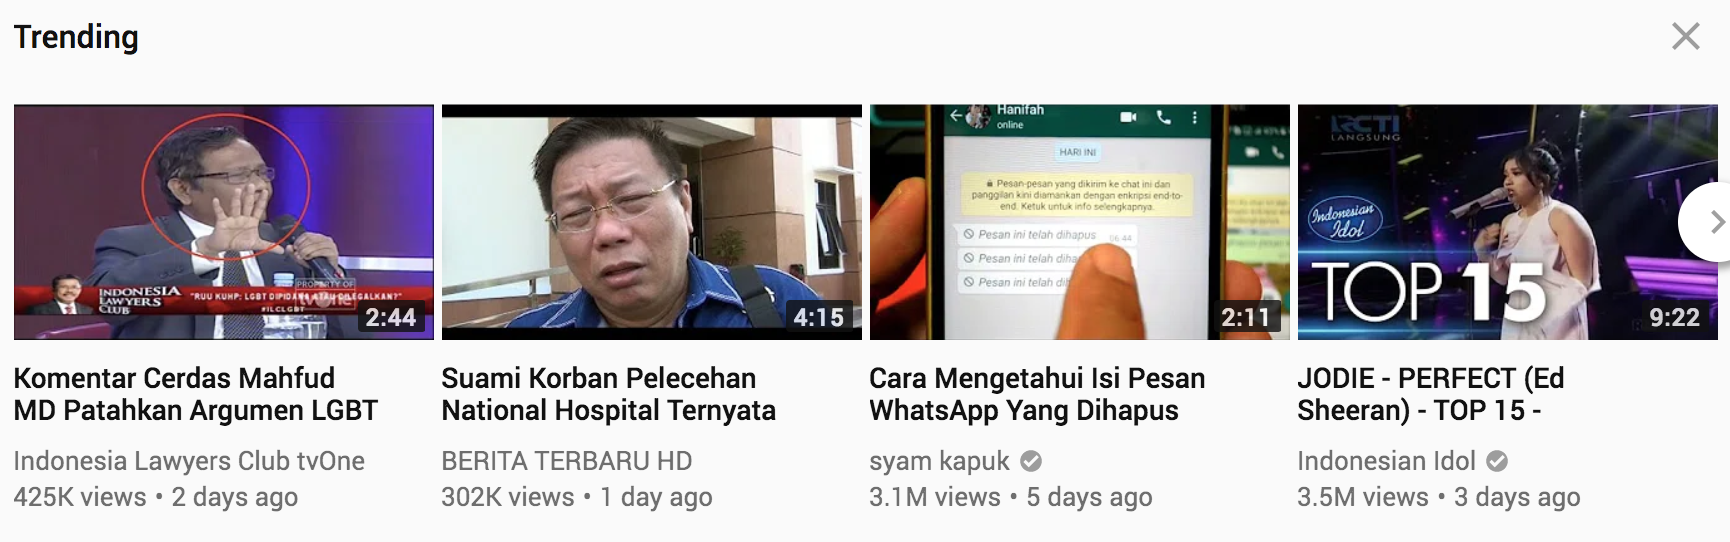
\includegraphics{trending.png}

\hypertarget{training-objectives}{%
\subsection{Training Objectives}\label{training-objectives}}

The primary objective of this course is to provide a fun and hands-on
session to help participants gain full proficiency in data visualization
systems and tools. You will learn to create compelling narratives by
combining charting elements with a rich grammar under the guidance of
the lead instructor and our team of teaching assistants.

\begin{itemize}
\item
  \textbf{Plotting Essential}
\item
  Revision: Built-in Plotting Functionalities\\
\item
  Revision: Scatterplot, Histogram, Line and Column Bars\\
\item
  Axis, Title and Panel Styles\\
\item
  Grammar of Graphics\\
\item
  \texttt{ggplot2} Basics
\item
  \textbf{Plotting Better}\\
\item
  Using Themes\\
\item
  Multi-dimensional Faceting\\
\item
  Visualizing Geo-Spatial Data with \texttt{leaflet}
\item
  Lattice Plotting system
\end{itemize}

By the end of the workshop, Academy students can choose to complete
either of the Learn-By-Building modules as their graded assignment:

\textbf{Ready for Publication}\\
Applying what you've learned, create a visualization that is polished
with the appropriate annotations, aesthetics and some simple commentary.
This can be any visualization using the YouTube dataset, but it should
communicate a story.

\textbf{Interactive Map}\\
Create a web page with an interactive map embedded on it. Use a custom
icon for the map markers to represent business locations, and show
details about each location pin (``markers'') upon user's interaction.

This graded assignment is worth \textbf{(2) Points}.

\hypertarget{plotting-essentials}{%
\section{Plotting Essentials}\label{plotting-essentials}}

R as a statistical computing environment packs a generous amount of
tools allowing us to reshape, clean and visualize our data through its
built-in capabilities. In the first part of this coursebook, we'll take
a look at many of these capabilities and learn how to incorporate these
into our day-to-day data science work.

In the second part of this coursebook, we'll shift our focus onto
\texttt{ggplot}, a plotting system by Hadley Wickham. As you'll see in
this 3 days workshop, this plotting system is among the most popular
visualization tools today because of its power, extensibility and
simplicity (an unlikely combination).

To get started with plotting in R, let's start by reading our data into
the environment:

\begin{Shaded}
\begin{Highlighting}[]
\NormalTok{vids <-}\StringTok{ }\KeywordTok{read.csv}\NormalTok{(}\StringTok{"USvideos.csv"}\NormalTok{)}
\KeywordTok{names}\NormalTok{(vids)}
\end{Highlighting}
\end{Shaded}

\begin{verbatim}
##  [1] "trending_date"          "title"                  "channel_title"         
##  [4] "category_id"            "publish_time"           "views"                 
##  [7] "likes"                  "dislikes"               "comment_count"         
## [10] "comments_disabled"      "ratings_disabled"       "video_error_or_removed"
\end{verbatim}

Taking a quick peek at the \texttt{trending\_date} column reveals that
the date values are stored in a year-day-month format, with \texttt{.}
(dot) being the delimiter:

\begin{Shaded}
\begin{Highlighting}[]
\KeywordTok{head}\NormalTok{(vids}\OperatorTok{$}\NormalTok{trending_date)}
\end{Highlighting}
\end{Shaded}

\begin{verbatim}
## [1] "17.14.11" "17.14.11" "17.14.11" "17.14.11" "17.14.11" "17.14.11"
\end{verbatim}

Because these values follows the \texttt{yy.dd.mm} format, our data
processing steps would handle this format accordindly through the
\texttt{format} argument:

\begin{Shaded}
\begin{Highlighting}[]
\NormalTok{vids}\OperatorTok{$}\NormalTok{trending_date <-}\StringTok{ }\KeywordTok{as.Date}\NormalTok{(vids}\OperatorTok{$}\NormalTok{trending_date, }\DataTypeTok{format=}\StringTok{"%y.%d.%m"}\NormalTok{)}
\end{Highlighting}
\end{Shaded}

In real life, most date formats uses a combination that maps to the
following:

\begin{itemize}
\tightlist
\item
  \texttt{\%Y}: 4-digit year (1982)\\
\item
  \texttt{\%y}: 2-digit year (82)\\
\item
  \texttt{\%m}: 2-digit month (01)\\
\item
  \texttt{\%d}: 2-digit day of the month (13)\\
\item
  \texttt{\%A}: weekday (Wednesday)\\
\item
  \texttt{\%a}: abbreviated weekday (Wed)\\
\item
  \texttt{\%B}: month (January)\\
\item
  \texttt{\%b}: abbreviated month (Jan)
\end{itemize}

You should follow your lead instructor on a few in-classroom practice to
increase your familiarity with the \texttt{as.Date()} function, as
processing dates are a fairly common process in many data analysis
routines:

\begin{Shaded}
\begin{Highlighting}[]
\CommentTok{# Demo: }
\KeywordTok{as.Date}\NormalTok{(}\StringTok{"Aug 30,2020"}\NormalTok{, }\DataTypeTok{format =} \StringTok{"%b %d,%Y"}\NormalTok{)}

\CommentTok{# Dive Deeper (complete the following):}
\KeywordTok{as.Date}\NormalTok{(}\StringTok{"30aug20"}\NormalTok{, }\DataTypeTok{format =}\NormalTok{ ___)}
\KeywordTok{as.Date}\NormalTok{(}\StringTok{"2020-08-30"}\NormalTok{, }\DataTypeTok{format =}\NormalTok{ ___)}
\KeywordTok{as.Date}\NormalTok{(}\StringTok{"08.30.2020"}\NormalTok{, }\DataTypeTok{format =}\NormalTok{ ___)}
\end{Highlighting}
\end{Shaded}

The raw dataset does not have the proper names for each category, but
identify them by an ``id'' instead. The following code chunk
``switches'' them by ``id'' and also convert that to a factor. We will
also convert our video titles to a character vector:

\begin{Shaded}
\begin{Highlighting}[]
\NormalTok{vids}\OperatorTok{$}\NormalTok{category_id <-}\StringTok{ }\KeywordTok{sapply}\NormalTok{(}\KeywordTok{as.character}\NormalTok{(vids}\OperatorTok{$}\NormalTok{category_id), }\ControlFlowTok{switch}\NormalTok{, }
                           \StringTok{"1"}\NormalTok{ =}\StringTok{ "Film and Animation"}\NormalTok{,}
                           \StringTok{"2"}\NormalTok{ =}\StringTok{ "Autos and Vehicles"}\NormalTok{, }
                           \StringTok{"10"}\NormalTok{ =}\StringTok{ "Music"}\NormalTok{, }
                           \StringTok{"15"}\NormalTok{ =}\StringTok{ "Pets and Animals"}\NormalTok{, }
                           \StringTok{"17"}\NormalTok{ =}\StringTok{ "Sports"}\NormalTok{,}
                           \StringTok{"19"}\NormalTok{ =}\StringTok{ "Travel and Events"}\NormalTok{, }
                           \StringTok{"20"}\NormalTok{ =}\StringTok{ "Gaming"}\NormalTok{, }
                           \StringTok{"22"}\NormalTok{ =}\StringTok{ "People and Blogs"}\NormalTok{, }
                           \StringTok{"23"}\NormalTok{ =}\StringTok{ "Comedy"}\NormalTok{,}
                           \StringTok{"24"}\NormalTok{ =}\StringTok{ "Entertainment"}\NormalTok{, }
                           \StringTok{"25"}\NormalTok{ =}\StringTok{ "News and Politics"}\NormalTok{,}
                           \StringTok{"26"}\NormalTok{ =}\StringTok{ "Howto and Style"}\NormalTok{, }
                           \StringTok{"27"}\NormalTok{ =}\StringTok{ "Education"}\NormalTok{,}
                           \StringTok{"28"}\NormalTok{ =}\StringTok{ "Science and Technology"}\NormalTok{, }
                           \StringTok{"29"}\NormalTok{ =}\StringTok{ "Nonprofit and Activism"}\NormalTok{,}
                           \StringTok{"43"}\NormalTok{ =}\StringTok{ "Shows"}\NormalTok{)}

\NormalTok{vids}\OperatorTok{$}\NormalTok{category_id <-}\StringTok{ }\KeywordTok{as.factor}\NormalTok{(vids}\OperatorTok{$}\NormalTok{category_id)}
\end{Highlighting}
\end{Shaded}

And with that, the next thing we'll need to do is to convert the
\texttt{publish\_time} variable into a date-time class object. Because
we're analyzing trending YouTube videos in the US, it makes sense then
that we uses a timezone like New York for our analysis:

\begin{Shaded}
\begin{Highlighting}[]
\KeywordTok{as.POSIXct}\NormalTok{(}\KeywordTok{head}\NormalTok{(vids}\OperatorTok{$}\NormalTok{publish_time), }
           \DataTypeTok{format=}\StringTok{"%Y-%m-%dT%H:%M:%S"}\NormalTok{, }
           \DataTypeTok{tz=}\StringTok{"America/New_York"}\NormalTok{)}
\end{Highlighting}
\end{Shaded}

\begin{verbatim}
## [1] "2017-11-13 17:13:01 EST" "2017-11-13 07:30:00 EST"
## [3] "2017-11-12 19:05:24 EST" "2017-11-13 11:00:04 EST"
## [5] "2017-11-12 18:01:41 EST" "2017-11-13 19:07:23 EST"
\end{verbatim}

Once we've done a sanity check, we can go ahead and apply the conversion
to the whole column:

\begin{Shaded}
\begin{Highlighting}[]
\NormalTok{vids}\OperatorTok{$}\NormalTok{publish_time <-}\StringTok{ }\KeywordTok{as.POSIXct}\NormalTok{(vids}\OperatorTok{$}\NormalTok{publish_time, }
           \DataTypeTok{format=}\StringTok{"%Y-%m-%dT%H:%M:%S"}\NormalTok{, }
           \DataTypeTok{tz=}\StringTok{"America/New_York"}\NormalTok{)}
\end{Highlighting}
\end{Shaded}

Once we've done a sanity check, we can go ahead and apply the conversion
to the whole column:

\begin{Shaded}
\begin{Highlighting}[]
\NormalTok{vids}\OperatorTok{$}\NormalTok{publish_time <-}\StringTok{ }\KeywordTok{as.POSIXct}\NormalTok{(vids}\OperatorTok{$}\NormalTok{publish_time, }
           \DataTypeTok{format=}\StringTok{"%Y-%m-%dT%H:%M:%S"}\NormalTok{, }
           \DataTypeTok{tz=}\StringTok{"America/New_York"}\NormalTok{)}
\end{Highlighting}
\end{Shaded}

By this point you may be wondering if this could have been made simpler.
Allow me to introduce a popular package by the name of
\texttt{lubridate}. Using \texttt{lubridate}, instead of manually
specifying the format, you do it ``declaratively'', like the following:

\begin{Shaded}
\begin{Highlighting}[]
\NormalTok{date <-}\StringTok{  }\KeywordTok{c}\NormalTok{(}\StringTok{"20.30.8"}\NormalTok{, }\StringTok{"20.31.8"}\NormalTok{)}
\NormalTok{date2 <-}\StringTok{ }\KeywordTok{c}\NormalTok{(}\StringTok{"30-8-20"}\NormalTok{, }\StringTok{"31-8-20"}\NormalTok{)}
\NormalTok{date3 <-}\StringTok{ }\KeywordTok{c}\NormalTok{(}\StringTok{"2017-11-13 17:13:01 EST"}\NormalTok{)}

\CommentTok{# base R}
\KeywordTok{as.Date}\NormalTok{(date, }\DataTypeTok{format=}\StringTok{"%y.%d.%m"}\NormalTok{)}
\end{Highlighting}
\end{Shaded}

\begin{verbatim}
## [1] "2020-08-30" "2020-08-31"
\end{verbatim}

\begin{Shaded}
\begin{Highlighting}[]
\KeywordTok{as.Date}\NormalTok{(date2, }\DataTypeTok{format=}\StringTok{"%d-%m-%y"}\NormalTok{)}
\end{Highlighting}
\end{Shaded}

\begin{verbatim}
## [1] "2020-08-30" "2020-08-31"
\end{verbatim}

\begin{Shaded}
\begin{Highlighting}[]
\KeywordTok{as.POSIXct}\NormalTok{(date3, }\DataTypeTok{format=}\StringTok{"%Y-%m-%d %H:%M:%S"}\NormalTok{, }\DataTypeTok{tz=}\StringTok{"UTC"}\NormalTok{)}
\end{Highlighting}
\end{Shaded}

\begin{verbatim}
## [1] "2017-11-13 17:13:01 UTC"
\end{verbatim}

\begin{Shaded}
\begin{Highlighting}[]
\CommentTok{# lubridate equivalent:}
\KeywordTok{ydm}\NormalTok{(date)}
\end{Highlighting}
\end{Shaded}

\begin{verbatim}
## [1] "2020-08-30" "2020-08-31"
\end{verbatim}

\begin{Shaded}
\begin{Highlighting}[]
\KeywordTok{dmy}\NormalTok{(date2)}
\end{Highlighting}
\end{Shaded}

\begin{verbatim}
## [1] "2020-08-30" "2020-08-31"
\end{verbatim}

\begin{Shaded}
\begin{Highlighting}[]
\KeywordTok{ymd_hms}\NormalTok{(date3, }\DataTypeTok{tz=}\StringTok{"UTC"}\NormalTok{)}
\end{Highlighting}
\end{Shaded}

\begin{verbatim}
## [1] "2017-11-13 17:13:01 UTC"
\end{verbatim}

Observe how simple \texttt{lubridate} work with dates and time. In fact,
when we use \texttt{ymd}, \texttt{ymd\_hms} or one of its variants,
these functions recognize the patterns and will identify the right
separators as long as the order of formats is correct. These functions
will also parse dates correctly even when the input contain differently
formatted dates!

Let's see a few more things that \texttt{lubridate} can do. I'll subset
the data for the most popular trending video (by number of views) and
we'll extract information from the \texttt{trending\_date} of the most
popular trending video:

\begin{Shaded}
\begin{Highlighting}[]
\NormalTok{most <-}\StringTok{ }\NormalTok{vids[vids}\OperatorTok{$}\NormalTok{views }\OperatorTok{==}\StringTok{ }\KeywordTok{max}\NormalTok{(vids}\OperatorTok{$}\NormalTok{views),]}
\KeywordTok{year}\NormalTok{(most}\OperatorTok{$}\NormalTok{trending_date)}
\end{Highlighting}
\end{Shaded}

\begin{verbatim}
## [1] 2017
\end{verbatim}

\begin{Shaded}
\begin{Highlighting}[]
\KeywordTok{month}\NormalTok{(most}\OperatorTok{$}\NormalTok{trending_date)}
\end{Highlighting}
\end{Shaded}

\begin{verbatim}
## [1] 12
\end{verbatim}

\begin{Shaded}
\begin{Highlighting}[]
\KeywordTok{day}\NormalTok{(most}\OperatorTok{$}\NormalTok{trending_date)}
\end{Highlighting}
\end{Shaded}

\begin{verbatim}
## [1] 14
\end{verbatim}

We will also go ahead and create three new variables for our data frame,
storing the hours, period of the day, and the day of the week of each
video at the time of publish:

\begin{Shaded}
\begin{Highlighting}[]
\NormalTok{vids}\OperatorTok{$}\NormalTok{publish_hour <-}\StringTok{ }\KeywordTok{hour}\NormalTok{(vids}\OperatorTok{$}\NormalTok{publish_time)}

\NormalTok{pw <-}\StringTok{ }\ControlFlowTok{function}\NormalTok{(x)\{}
    \ControlFlowTok{if}\NormalTok{(x }\OperatorTok{<}\StringTok{ }\DecValTok{8}\NormalTok{)\{}
\NormalTok{      x <-}\StringTok{ "12am to 8am"}
\NormalTok{    \}}\ControlFlowTok{else} \ControlFlowTok{if}\NormalTok{(x }\OperatorTok{>=}\StringTok{ }\DecValTok{8} \OperatorTok{&}\StringTok{ }\NormalTok{x }\OperatorTok{<}\StringTok{ }\DecValTok{16}\NormalTok{)\{}
\NormalTok{      x <-}\StringTok{ "8am to 3pm"}
\NormalTok{    \}}\ControlFlowTok{else}\NormalTok{\{}
\NormalTok{      x <-}\StringTok{ "3pm to 12am"}
\NormalTok{    \}  }
\NormalTok{\}}

\NormalTok{vids}\OperatorTok{$}\NormalTok{publish_when <-}\StringTok{ }\KeywordTok{as.factor}\NormalTok{(}\KeywordTok{sapply}\NormalTok{(vids}\OperatorTok{$}\NormalTok{publish_hour, pw))}
\NormalTok{vids}\OperatorTok{$}\NormalTok{publish_wday <-}\StringTok{ }\KeywordTok{as.factor}\NormalTok{(}\KeywordTok{weekdays}\NormalTok{(vids}\OperatorTok{$}\NormalTok{publish_time))}
\end{Highlighting}
\end{Shaded}

While the \texttt{publish\_wday} is now a factor, we can also arrange it
so our plots later will display them in our desired order:

\begin{Shaded}
\begin{Highlighting}[]
\NormalTok{vids}\OperatorTok{$}\NormalTok{publish_wday <-}\StringTok{ }\KeywordTok{ordered}\NormalTok{(vids}\OperatorTok{$}\NormalTok{publish_wday, }\DataTypeTok{levels=}\KeywordTok{c}\NormalTok{(}\StringTok{"Monday"}\NormalTok{, }\StringTok{"Tuesday"}\NormalTok{, }\StringTok{"Wednesday"}\NormalTok{, }\StringTok{"Thursday"}\NormalTok{, }\StringTok{"Friday"}\NormalTok{, }\StringTok{"Saturday"}\NormalTok{, }\StringTok{"Sunday"}\NormalTok{))}
\end{Highlighting}
\end{Shaded}

We'll also go ahead and convert some of the variables into numeric
variables as and where appropriate:

\begin{Shaded}
\begin{Highlighting}[]
\NormalTok{vids[,}\KeywordTok{c}\NormalTok{(}\StringTok{"views"}\NormalTok{, }\StringTok{"likes"}\NormalTok{, }\StringTok{"dislikes"}\NormalTok{, }\StringTok{"comment_count"}\NormalTok{)] <-}\StringTok{ }\KeywordTok{lapply}\NormalTok{(vids[,}\KeywordTok{c}\NormalTok{(}\StringTok{"views"}\NormalTok{, }\StringTok{"likes"}\NormalTok{, }\StringTok{"dislikes"}\NormalTok{, }\StringTok{"comment_count"}\NormalTok{)], as.numeric)}
\end{Highlighting}
\end{Shaded}

Hopefully up to this point, none of the above data transformation and
cleansing process looks too unfamiliar for you! If you do need a
refresher, refer to the Programming for Data Science coursebook - we're
really applying many of the same ideas to a new dataset, and so you
should feel somewhat comfortable up to this point of the course :)

\texttt{vids} has 13400 records of trending videos, but there are many
videos that were trending for a few days and we really only have a
collection of 2,986 unique videos. On a very broad average, each video
was trending for \textasciitilde{}4.5 days.

Let's create a dataframe, call it \texttt{vids.u} that takes only the
first observation of each \texttt{vids.title} within the data.
\texttt{match} returns a vector of the positions of matches of its first
argument in its second:

\begin{Shaded}
\begin{Highlighting}[]
\NormalTok{vids.u <-}\StringTok{ }\NormalTok{vids[}\KeywordTok{match}\NormalTok{(}\KeywordTok{unique}\NormalTok{(vids}\OperatorTok{$}\NormalTok{title), vids}\OperatorTok{$}\NormalTok{title),]}
\end{Highlighting}
\end{Shaded}

We'll also create one more variable \texttt{timetotrend} to measure the
time it takes for a video to become ``trending'':

\begin{Shaded}
\begin{Highlighting}[]
\NormalTok{vids.u}\OperatorTok{$}\NormalTok{timetotrend <-}\StringTok{ }\NormalTok{vids.u}\OperatorTok{$}\NormalTok{trending_date }\OperatorTok{-}\StringTok{ }\KeywordTok{as.Date}\NormalTok{(vids.u}\OperatorTok{$}\NormalTok{publish_time)}
\NormalTok{vids.u}\OperatorTok{$}\NormalTok{timetotrend <-}\StringTok{ }\KeywordTok{as.factor}\NormalTok{(}\KeywordTok{ifelse}\NormalTok{(vids.u}\OperatorTok{$}\NormalTok{timetotrend }\OperatorTok{<=}\StringTok{ }\DecValTok{7}\NormalTok{, vids.u}\OperatorTok{$}\NormalTok{timetotrend, }\StringTok{"8+"}\NormalTok{))}
\end{Highlighting}
\end{Shaded}

With these done, we'll move into the exciting part of this workshop:
plotting!

\hypertarget{base-plotting-and-statistical-plots}{%
\subsection{Base Plotting and Statistical
Plots}\label{base-plotting-and-statistical-plots}}

Statistical plots helps us visually inspect our dataset and there are
numerous ways to achieve that in R. The simplest of which is through the
\texttt{plot()} function. In the following code we create two vectors,
\texttt{x} and \texttt{y}, and created a plot:

\begin{Shaded}
\begin{Highlighting}[]
\KeywordTok{plot}\NormalTok{(}\KeywordTok{as.factor}\NormalTok{(vids.u}\OperatorTok{$}\NormalTok{publish_hour), vids.u}\OperatorTok{$}\NormalTok{likes}\OperatorTok{/}\NormalTok{vids.u}\OperatorTok{$}\NormalTok{views)}
\end{Highlighting}
\end{Shaded}

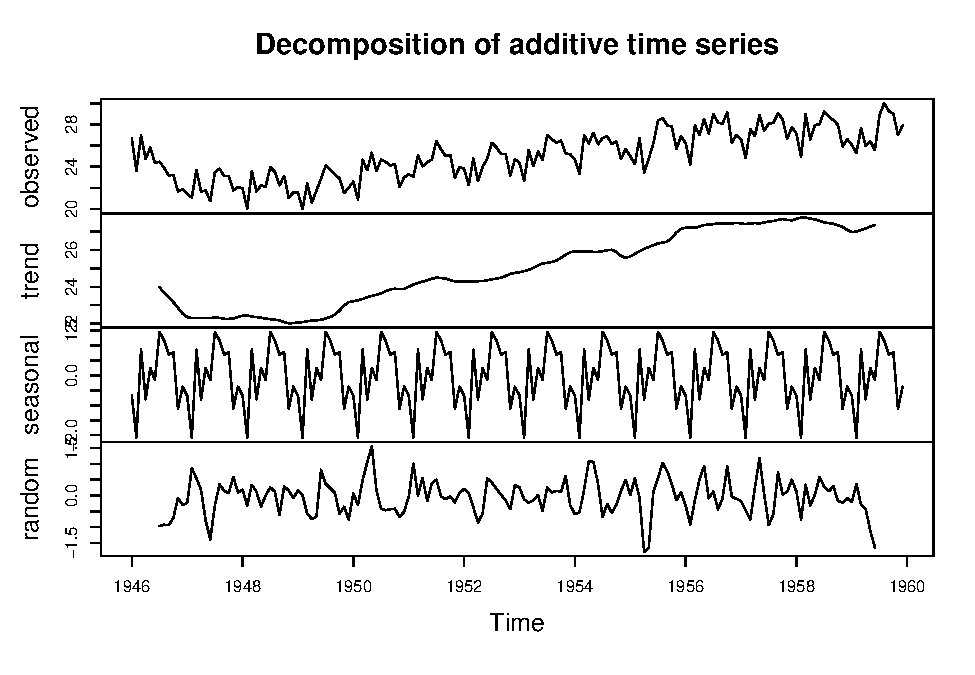
\includegraphics{dv_files/figure-latex/unnamed-chunk-17-1.pdf}

The above gives us a boxplot that compares the ``likes ratio'' across
different period of the day. We want to observe if there is any
correlation between the likes-to-view percentage and the period of time
when the video was published. As expected, we did not find any obvious
patterns, in part because this compares the ``likes'' a video have on
the first day of it being ``trending'' and the hour when it was
published onto YouTube. In a sense, any kind of effect the hour variable
can have has been adjusted for (or significantly reduced) by the noise
between these two events.

\texttt{plot()} knows how to pick sensible defaults based on the input
vector it was given. To illustrate this point, I'll subset the data to
take only trending videos within the Autos, Gaming and Travel industry
(every women's favorite 3 things):

\begin{Shaded}
\begin{Highlighting}[]
\NormalTok{vids.agt <-}\StringTok{ }\NormalTok{vids.u[vids.u}\OperatorTok{$}\NormalTok{category_id }\OperatorTok{==}\StringTok{ "Autos and Vehicles"} \OperatorTok{|}
\StringTok{                     }\NormalTok{vids.u}\OperatorTok{$}\NormalTok{category_id }\OperatorTok{==}\StringTok{ "Gaming"} \OperatorTok{|}\StringTok{ }
\StringTok{                     }\NormalTok{vids.u}\OperatorTok{$}\NormalTok{category_id }\OperatorTok{==}\StringTok{ "Travel and Events"}\NormalTok{, ]}
\end{Highlighting}
\end{Shaded}

And notice that as we call \texttt{plot} now on that subset, instead of
a boxplot, the \texttt{plot()} function knows that we're plotting two
numeric variables and creates a scatterplot for us instead:

\begin{Shaded}
\begin{Highlighting}[]
\KeywordTok{plot}\NormalTok{(vids.agt}\OperatorTok{$}\NormalTok{likes, vids.agt}\OperatorTok{$}\NormalTok{dislikes)}
\end{Highlighting}
\end{Shaded}

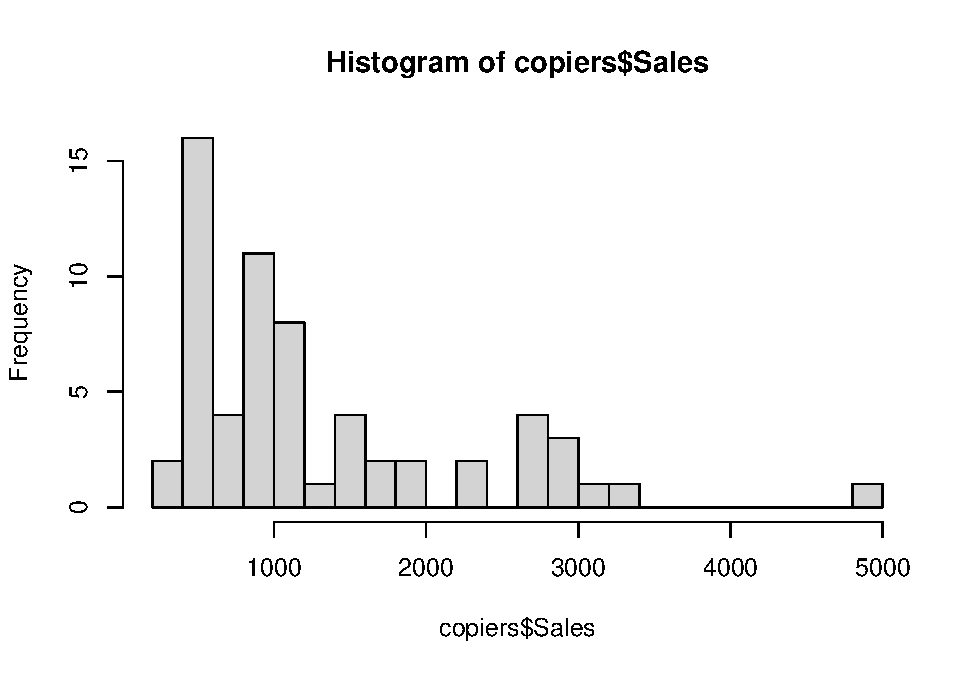
\includegraphics{dv_files/figure-latex/unnamed-chunk-19-1.pdf}

We'll drop the empty levels from our \texttt{category\_id} variable, and
also create two new variables that measure the likes and dislikes per
video view for each observation:

\begin{Shaded}
\begin{Highlighting}[]
\NormalTok{vids.agt}\OperatorTok{$}\NormalTok{category_id <-}\StringTok{ }\KeywordTok{factor}\NormalTok{(vids.agt}\OperatorTok{$}\NormalTok{category_id)}
\NormalTok{vids.agt}\OperatorTok{$}\NormalTok{likesp <-}\StringTok{ }\NormalTok{vids.agt}\OperatorTok{$}\NormalTok{likes}\OperatorTok{/}\NormalTok{vids.agt}\OperatorTok{$}\NormalTok{views}
\NormalTok{vids.agt}\OperatorTok{$}\NormalTok{dislikesp <-}\StringTok{ }\NormalTok{vids.agt}\OperatorTok{$}\NormalTok{dislikes}\OperatorTok{/}\NormalTok{vids.agt}\OperatorTok{$}\NormalTok{views}
\end{Highlighting}
\end{Shaded}

Our earlier scatterplot really isn't very informative or even pleasant
to look at. The key, as it is with data visualization in general, is to
have our plot be effective. A plot that is effective complements how
human visual perception works. The scatterplot is ineffective because it
could be communicating more with less ``visual clutter'' at the bottom
left.

An approach to fix that is by coloring the plots. In the following code
chunk, the first line is identical to the code that produces the
scatterplot above except for one addition, the \texttt{col} (color)
parameter. We mapped the color parameter to the category so the points
are colored accordingly.

I've also added a dashed line (\texttt{lty}) with a width of 2
(\texttt{lwd=2}) to show that the correlation between the likes-to-view
and dislikes-to-view ratio.

Finally, I added a legend for our plot to show how the colors of our
scatterplot points map to each level of our \texttt{category\_id}
variable.

Here's the code:

\begin{Shaded}
\begin{Highlighting}[]
\KeywordTok{plot}\NormalTok{(vids.agt}\OperatorTok{$}\NormalTok{likesp, vids.agt}\OperatorTok{$}\NormalTok{dislikesp, }\DataTypeTok{col=}\NormalTok{vids.agt}\OperatorTok{$}\NormalTok{category_id, }\DataTypeTok{pch=}\DecValTok{19}\NormalTok{)}
\KeywordTok{abline}\NormalTok{(}\KeywordTok{lm}\NormalTok{(vids.agt}\OperatorTok{$}\NormalTok{dislikesp }\OperatorTok{~}\StringTok{ }\NormalTok{vids.agt}\OperatorTok{$}\NormalTok{likesp), }\DataTypeTok{col=}\DecValTok{8}\NormalTok{, }\DataTypeTok{lwd=}\DecValTok{2}\NormalTok{, }\DataTypeTok{lty=}\DecValTok{2}\NormalTok{)}
\KeywordTok{legend}\NormalTok{(}\StringTok{"topright"}\NormalTok{, }\DataTypeTok{legend=}\KeywordTok{levels}\NormalTok{(vids.agt}\OperatorTok{$}\NormalTok{category_id), }\DataTypeTok{fill=}\DecValTok{1}\OperatorTok{:}\DecValTok{3}\NormalTok{)}
\end{Highlighting}
\end{Shaded}

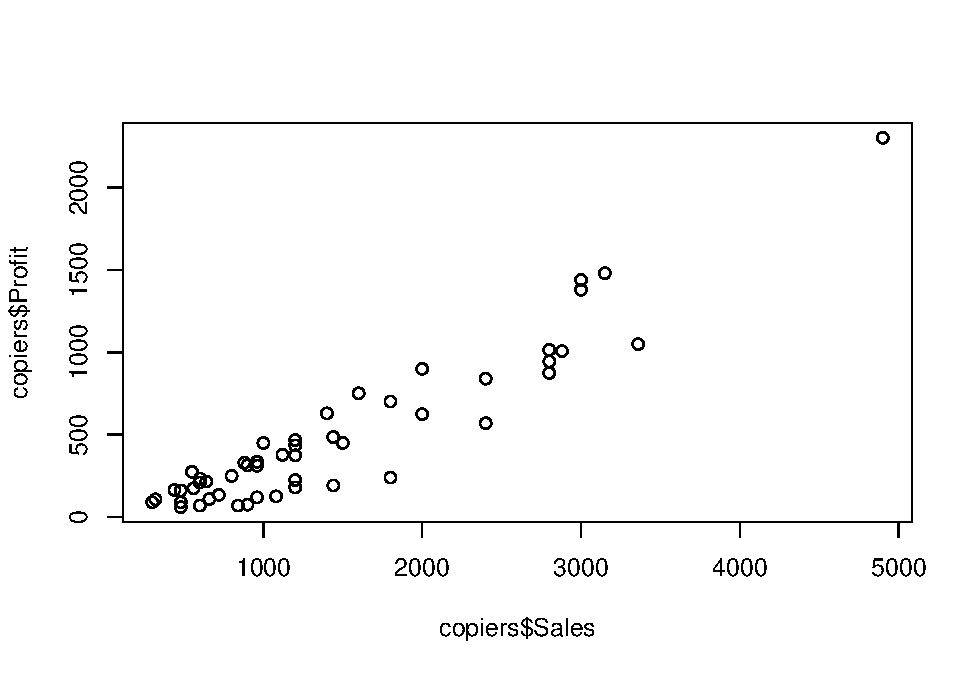
\includegraphics{dv_files/figure-latex/unnamed-chunk-21-1.pdf}

With \texttt{plot}, the default for two numerical variables is to plot a
scatterplot, but we can override the default parameters with the
\texttt{type} argument. The following code chunk is identical to the one
above, except for the \texttt{type="h"} addition:

\begin{Shaded}
\begin{Highlighting}[]
\KeywordTok{plot}\NormalTok{(vids.agt}\OperatorTok{$}\NormalTok{likesp, vids.agt}\OperatorTok{$}\NormalTok{dislikesp, }\DataTypeTok{col=}\NormalTok{vids.agt}\OperatorTok{$}\NormalTok{category_id, }\DataTypeTok{type=}\StringTok{"h"}\NormalTok{)}
\KeywordTok{abline}\NormalTok{(}\KeywordTok{lm}\NormalTok{(vids.agt}\OperatorTok{$}\NormalTok{dislikesp }\OperatorTok{~}\StringTok{ }\NormalTok{vids.agt}\OperatorTok{$}\NormalTok{likesp), }\DataTypeTok{col=}\DecValTok{8}\NormalTok{, }\DataTypeTok{lwd=}\DecValTok{2}\NormalTok{, }\DataTypeTok{lty=}\DecValTok{2}\NormalTok{)}
\KeywordTok{legend}\NormalTok{(}\StringTok{"topright"}\NormalTok{, }\DataTypeTok{legend=}\KeywordTok{levels}\NormalTok{(vids.agt}\OperatorTok{$}\NormalTok{category_id), }\DataTypeTok{fill=}\DecValTok{1}\OperatorTok{:}\DecValTok{3}\NormalTok{)}
\end{Highlighting}
\end{Shaded}

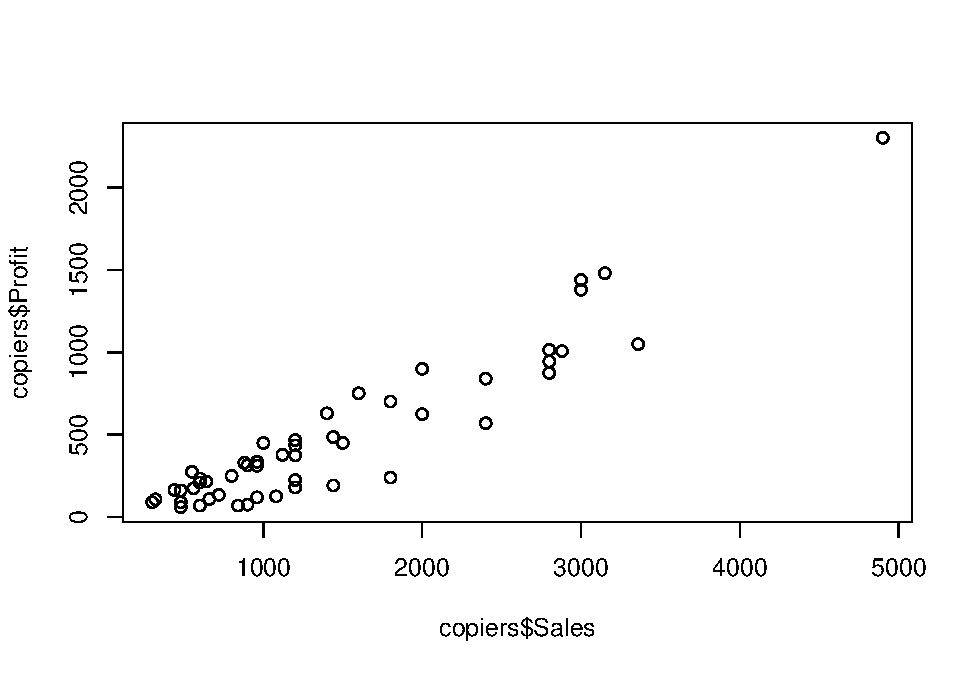
\includegraphics{dv_files/figure-latex/unnamed-chunk-22-1.pdf}

Apart from using \texttt{plot()}, we can also create statistical plots
using functions such as \texttt{hist()}. \texttt{hist()} takes a numeric
vector and creates a histogram:

\begin{Shaded}
\begin{Highlighting}[]
\KeywordTok{hist}\NormalTok{(vids.agt}\OperatorTok{$}\NormalTok{likesp)}
\end{Highlighting}
\end{Shaded}

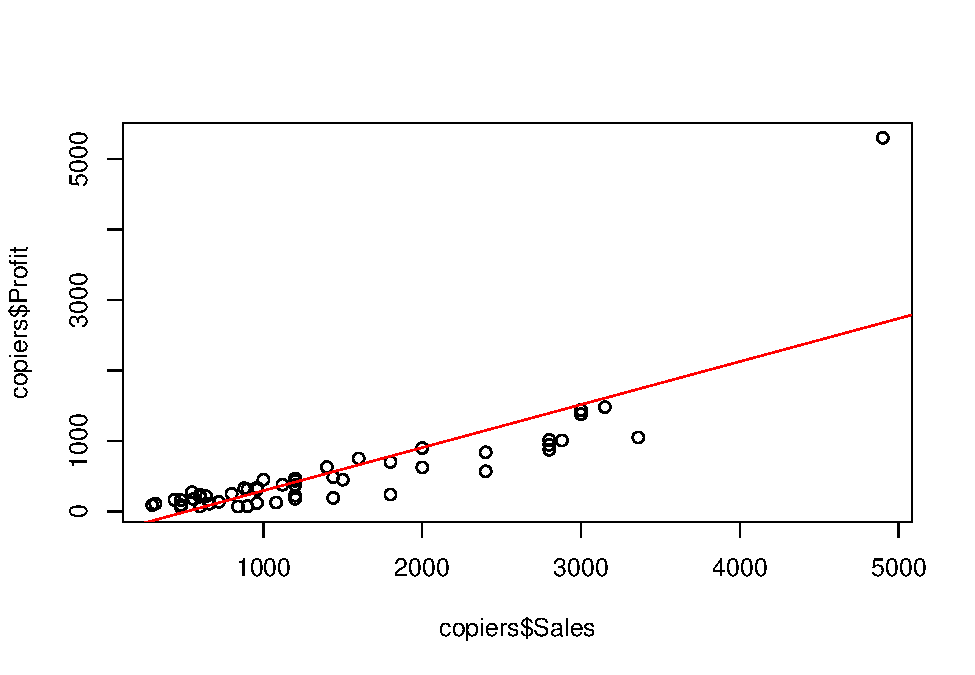
\includegraphics{dv_files/figure-latex/unnamed-chunk-23-1.pdf}

We can additionally use the \texttt{breaks} argument to control the
number of bins if we were not satisfied with the default values:

\begin{Shaded}
\begin{Highlighting}[]
\KeywordTok{hist}\NormalTok{(vids.agt}\OperatorTok{$}\NormalTok{likesp, }\DataTypeTok{breaks=}\DecValTok{20}\NormalTok{)}
\end{Highlighting}
\end{Shaded}

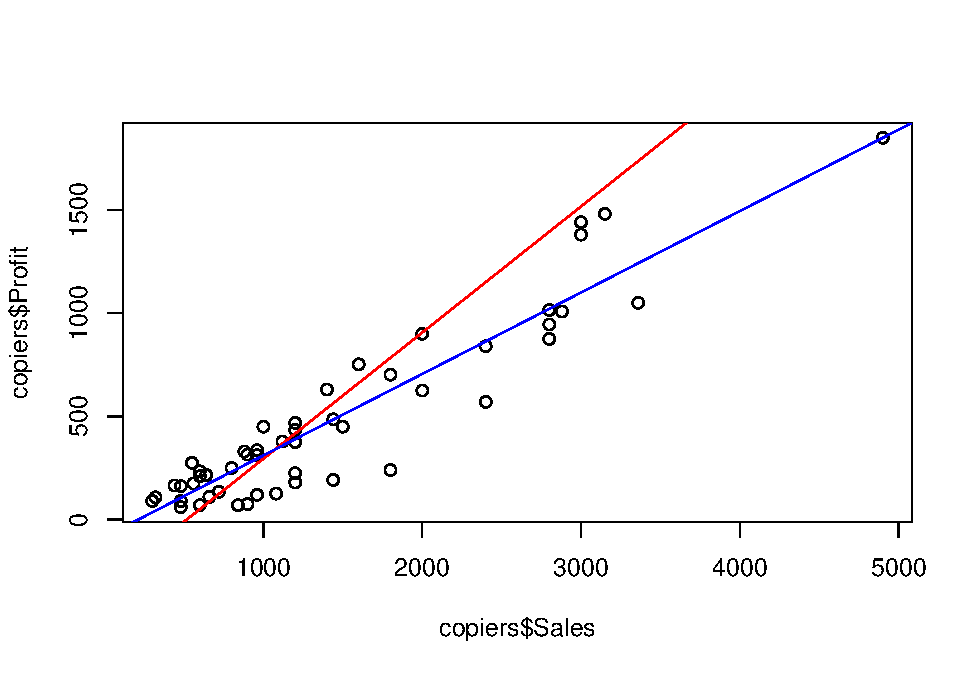
\includegraphics{dv_files/figure-latex/unnamed-chunk-24-1.pdf}

Just like how we can add \texttt{abline} onto our plot, we can add
graphical elements like \texttt{lines} onto this histogram too. In fact,
let's do that and also use the \texttt{main} argument to give our plot a
new main title:

\begin{Shaded}
\begin{Highlighting}[]
\KeywordTok{hist}\NormalTok{(vids.agt}\OperatorTok{$}\NormalTok{likesp, }
     \DataTypeTok{breaks=}\DecValTok{20}\NormalTok{, }
     \DataTypeTok{ylim=}\KeywordTok{c}\NormalTok{(}\DecValTok{0}\NormalTok{, }\DecValTok{20}\NormalTok{), }
     \DataTypeTok{col=}\StringTok{"lightblue"}\NormalTok{, }
     \DataTypeTok{main=}\StringTok{"Distribution of likes-per-view"}\NormalTok{)}
\KeywordTok{lines}\NormalTok{(}\KeywordTok{density}\NormalTok{(vids.agt}\OperatorTok{$}\NormalTok{likesp), }\DataTypeTok{col=}\StringTok{"darkblue"}\NormalTok{)}
\end{Highlighting}
\end{Shaded}

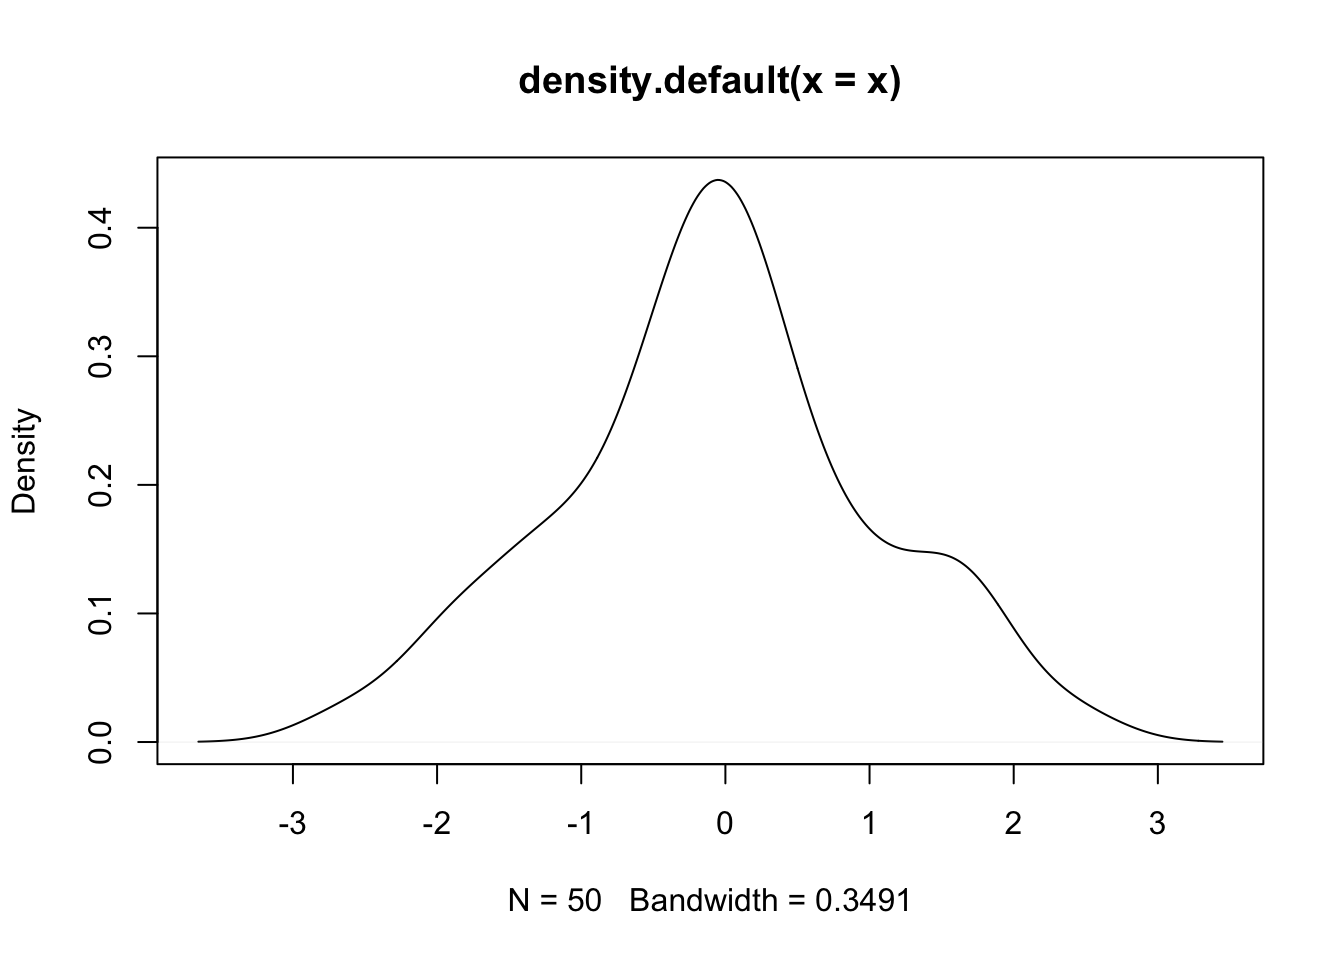
\includegraphics{dv_files/figure-latex/unnamed-chunk-25-1.pdf}

While base plot can be very simple to use, they can be effective too. In
fact, with the use of proper coloring, annotation and a little care on
the aesthetic touches, you can communicate a lot in a graph using just
R's built-in plotting system.

In the following code chunk I'm subsetting from \texttt{vids.agt} only
trending videos that have more than 10,000 likes and order it by the
likes-to-view variable. I added a new variable, \texttt{col} to this new
dataframe to be used in my following plot:

\begin{Shaded}
\begin{Highlighting}[]
\NormalTok{vids.ags <-}\StringTok{ }\NormalTok{vids.agt[vids.agt}\OperatorTok{$}\NormalTok{likes }\OperatorTok{>}\StringTok{ }\DecValTok{10000}\NormalTok{, ]}
\NormalTok{vids.ags <-}\StringTok{ }\NormalTok{vids.ags[}\KeywordTok{order}\NormalTok{(vids.ags}\OperatorTok{$}\NormalTok{likesp), ]}

\CommentTok{# create color specifications for our dotchart}
\NormalTok{vids.ags}\OperatorTok{$}\NormalTok{col[vids.ags}\OperatorTok{$}\NormalTok{category_id }\OperatorTok{==}\StringTok{ "Autos and Vehicles"}\NormalTok{] <-}\StringTok{ "goldenrod4"}
\NormalTok{vids.ags}\OperatorTok{$}\NormalTok{col[vids.ags}\OperatorTok{$}\NormalTok{category_id }\OperatorTok{==}\StringTok{ "Gaming"}\NormalTok{] <-}\StringTok{ "dodgerblue4"}
\NormalTok{vids.ags}\OperatorTok{$}\NormalTok{col[vids.ags}\OperatorTok{$}\NormalTok{category_id }\OperatorTok{==}\StringTok{ "Travel and Events"}\NormalTok{] <-}\StringTok{ "firebrick4"}
\end{Highlighting}
\end{Shaded}

We're going to create a dot chart (or a Cleveland's Dot Plot) by
graphing the likes to view ratio of each trending video in the
\texttt{vids.ags} dataframe, map \texttt{channel\_title} to the labels
and group these labels by \texttt{category\_id}.

\begin{Shaded}
\begin{Highlighting}[]
\KeywordTok{dotchart}\NormalTok{(vids.ags}\OperatorTok{$}\NormalTok{likesp, }\DataTypeTok{labels=}\NormalTok{vids.ags}\OperatorTok{$}\NormalTok{channel_title, }\DataTypeTok{cex=}\NormalTok{.}\DecValTok{7}\NormalTok{, }\DataTypeTok{pch=}\DecValTok{19}\NormalTok{, }\DataTypeTok{groups=}\NormalTok{vids.ags}\OperatorTok{$}\NormalTok{category_id, }\DataTypeTok{col=}\NormalTok{vids.ags}\OperatorTok{$}\NormalTok{col)}
\end{Highlighting}
\end{Shaded}

\begin{verbatim}
## Warning in strwidth(labels, "inch"): conversion failure on 'Pok̩mon GO' in
## 'mbcsToSbcs': dot substituted for <cc>
\end{verbatim}

\begin{verbatim}
## Warning in strwidth(labels, "inch"): conversion failure on 'Pok̩mon GO' in
## 'mbcsToSbcs': dot substituted for <a9>
\end{verbatim}

\begin{verbatim}
## Warning in strwidth(labels, "inch"): conversion failure on 'The Official Pok̩mon
## YouTube Channel' in 'mbcsToSbcs': dot substituted for <cc>
\end{verbatim}

\begin{verbatim}
## Warning in strwidth(labels, "inch"): conversion failure on 'The Official Pok̩mon
## YouTube Channel' in 'mbcsToSbcs': dot substituted for <a9>
\end{verbatim}

\begin{verbatim}
## Warning in mtext(labels[o], side = 2, line = loffset, at = y, adj = 0, col =
## color, : conversion failure on 'Pok̩mon GO' in 'mbcsToSbcs': dot substituted for
## <cc>
\end{verbatim}

\begin{verbatim}
## Warning in mtext(labels[o], side = 2, line = loffset, at = y, adj = 0, col =
## color, : conversion failure on 'Pok̩mon GO' in 'mbcsToSbcs': dot substituted for
## <a9>
\end{verbatim}

\begin{verbatim}
## Warning in mtext(labels[o], side = 2, line = loffset, at = y, adj = 0, col
## = color, : conversion failure on 'The Official Pok̩mon YouTube Channel' in
## 'mbcsToSbcs': dot substituted for <cc>
\end{verbatim}

\begin{verbatim}
## Warning in mtext(labels[o], side = 2, line = loffset, at = y, adj = 0, col
## = color, : conversion failure on 'The Official Pok̩mon YouTube Channel' in
## 'mbcsToSbcs': dot substituted for <a9>
\end{verbatim}

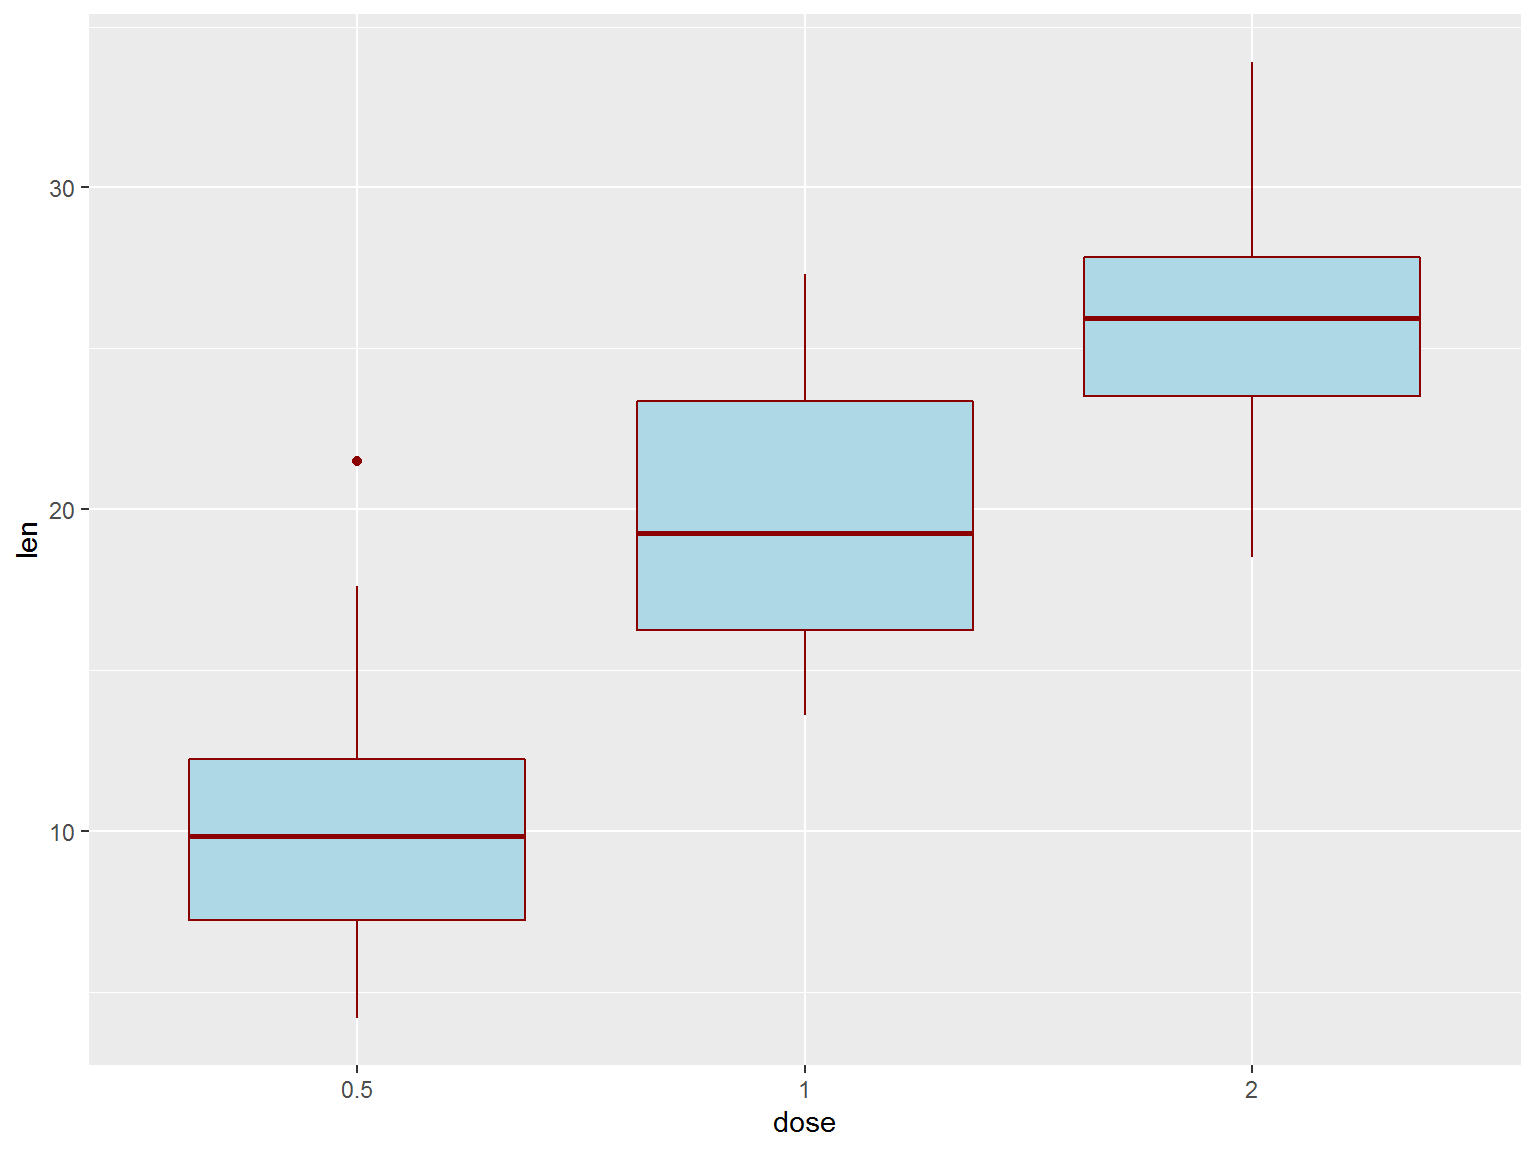
\includegraphics{dv_files/figure-latex/unnamed-chunk-27-1.pdf}

With this we see that between groups, the likes to view proportion
(we'll call it ``likeability'' from now on) of Autos and Vehicles are
rather similar with Travel and Events.However, for gaming videos we do
see a larger variance in that the top video by likeability is close to
0.13, more than 6 times difference to that of other trending videos in
this category. We also observe the rough mean likeability within groups,
as well as between them. We would expect Travel and Events videos to
have \textasciitilde{}4 likes per 100 views, and Gaming videos to have
more than that due to the positive skew we observe from above.

Let's talk about another kind of plot, one that most statisticians find
cringeworthy for it's undeserved popularity and prevalence in the
workplace. Yes, it is the pie chart. In R's official documentation, the
pie chart is criticized as being ``a very bad way of displaying
information {[}because{]} the eye is good at judging linear measures and
bad at judging relative areas''. Almost any data that can be represented
in a pie chart can be illustrated with a bar chart or dot
chart\footnote{Full Note on pie charts from the official R
  Documentation:\\
  "Pie charts are a very bad way of displaying information. The eye is
  good at judging linear measures and bad at judging relative areas. A
  bar chart or dot chart is a preferable way of displaying this type of
  data.}.

If you insist on creating one, here's the code (I've added some colors
to make it easier to get a grasp of the measures):

\begin{Shaded}
\begin{Highlighting}[]
\KeywordTok{pie}\NormalTok{(}\KeywordTok{table}\NormalTok{(vids.ags}\OperatorTok{$}\NormalTok{publish_hour), }\DataTypeTok{labels=}\KeywordTok{names}\NormalTok{(}\KeywordTok{table}\NormalTok{(vids.ags}\OperatorTok{$}\NormalTok{publish_hour)), }\DataTypeTok{col=}\KeywordTok{topo.colors}\NormalTok{(}\DecValTok{24}\NormalTok{))}
\end{Highlighting}
\end{Shaded}

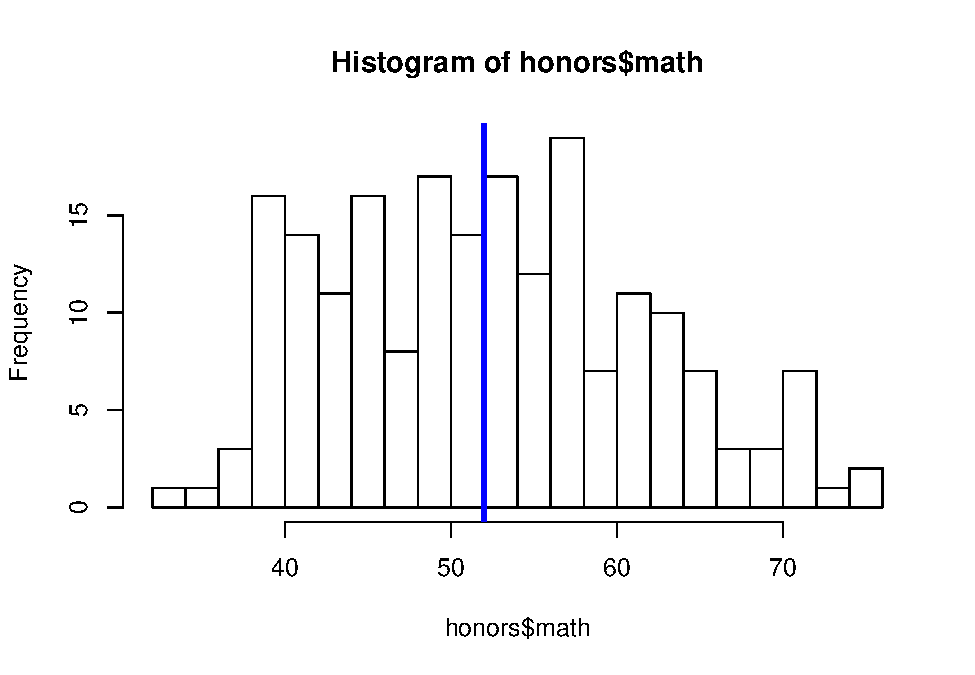
\includegraphics{dv_files/figure-latex/unnamed-chunk-28-1.pdf}

\hypertarget{grammar-of-graphics-in-r}{%
\subsection{Grammar of Graphics in R}\label{grammar-of-graphics-in-r}}

\hypertarget{the-motivation-of-ggplot2}{%
\subsubsection{The motivation of
ggplot2}\label{the-motivation-of-ggplot2}}

\texttt{ggplot2} is created by Hadley Wickham in 2005 as an
implementation of Lelad Wilkinson's Grammar of Graphics. The idea with
Grammar of Graphics is to create a formal model for data visualization,
by breaking down graphics into components that could be systematically
added or subtracted by the end user.

With \texttt{ggplot2}, plots may be created using \texttt{qplot()} where
arguments and defaults are handled similarly to the base plotting
system, or through \texttt{ggplot()} where user can add or alter plot
components layer-by-layer with a high level of modularity.

The last point is especially important because it allows the data
scientists to work with plots in a system that breaks up these different
tasks. Instead of a huge, conceptually flat list of parameters to
control every aspect of the plot's final outcome, this system makes
plotting a series of distinct task, each focused on one aspect of the
plot's final output.

Let us take a look at a simple example, drawing inspiration from the
Earthquake incident that happened in the south of Jakarta this week (as
of this writing). I've created a dataframe called \texttt{gempa}:

\begin{Shaded}
\begin{Highlighting}[]
\NormalTok{gempa <-}\StringTok{ }\KeywordTok{data.frame}\NormalTok{(}
  \DataTypeTok{x=}\KeywordTok{c}\NormalTok{(}\FloatTok{3.5}\NormalTok{,}\DecValTok{3}\NormalTok{,}\DecValTok{4}\NormalTok{,}\FloatTok{4.5}\NormalTok{,}\FloatTok{4.1}\NormalTok{),}
  \DataTypeTok{y=}\KeywordTok{c}\NormalTok{(}\DecValTok{12}\NormalTok{,}\DecValTok{14}\NormalTok{,}\FloatTok{12.4}\NormalTok{,}\FloatTok{12.5}\NormalTok{,}\DecValTok{14}\NormalTok{), }
  \DataTypeTok{size=}\KeywordTok{c}\NormalTok{(}\DecValTok{14}\NormalTok{,}\DecValTok{4}\NormalTok{,}\DecValTok{4}\NormalTok{,}\DecValTok{6}\NormalTok{,}\DecValTok{12}\NormalTok{)}
\NormalTok{)}
\end{Highlighting}
\end{Shaded}

And now I'll create a ggplot object using \texttt{ggplot()}. Because of
the range of my values, this plot will use that and create a plot with
these values on each scales (scales, by the way, can be thought of as
just the two axis right now). Note that we're just creating a blank plot
with no geometry elements (lines, points, etc) on it yet. We save this
object as \texttt{g}:

\begin{Shaded}
\begin{Highlighting}[]
\NormalTok{g <-}\StringTok{ }\KeywordTok{ggplot}\NormalTok{(gempa, }\KeywordTok{aes}\NormalTok{(}\DataTypeTok{x =}\NormalTok{ x, }\DataTypeTok{y =}\NormalTok{ y))}
\NormalTok{g}
\end{Highlighting}
\end{Shaded}

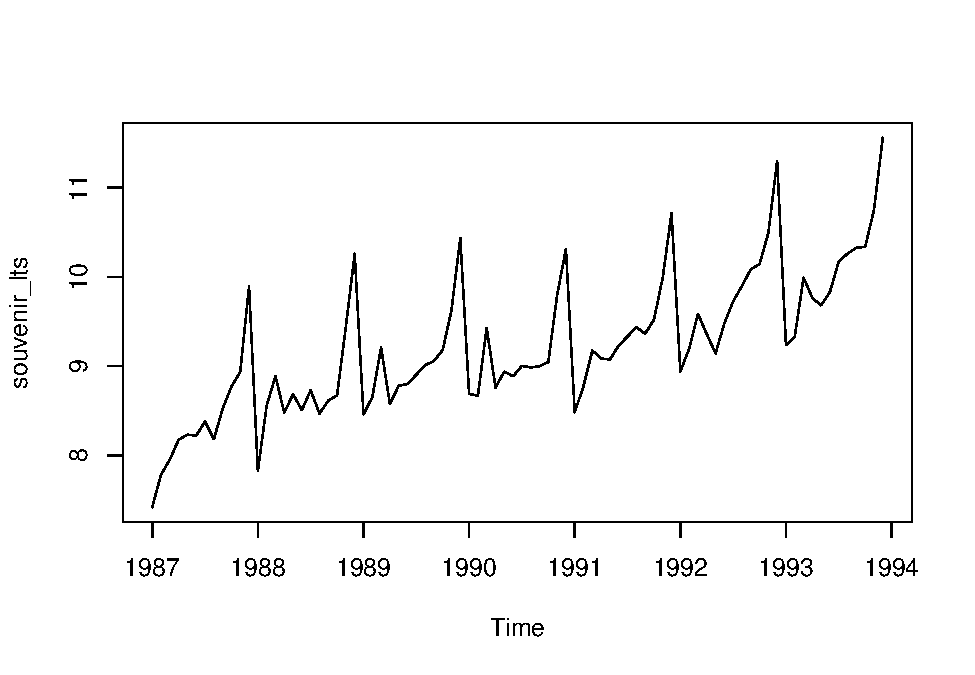
\includegraphics{dv_files/figure-latex/unnamed-chunk-30-1.pdf}

Notice how \texttt{ggplot()} takes two arguments: - The data - The
\texttt{aes} which allow us to specify our mapping of the x and y
variables so they are used accordingly by ggplot

Once we created our \texttt{ggplot} object (we named it \texttt{g}), we
can now add a layer onto it using \texttt{geom\_}. \texttt{geom} is
ggplot's way of handling geometry, i.e.~how the data are represented on
the plot. To illustrate this idea, let's add a geom\_point and then
print the resulting object:

\begin{Shaded}
\begin{Highlighting}[]
\NormalTok{g }\OperatorTok{+}\StringTok{ }\KeywordTok{geom_point}\NormalTok{()}
\end{Highlighting}
\end{Shaded}

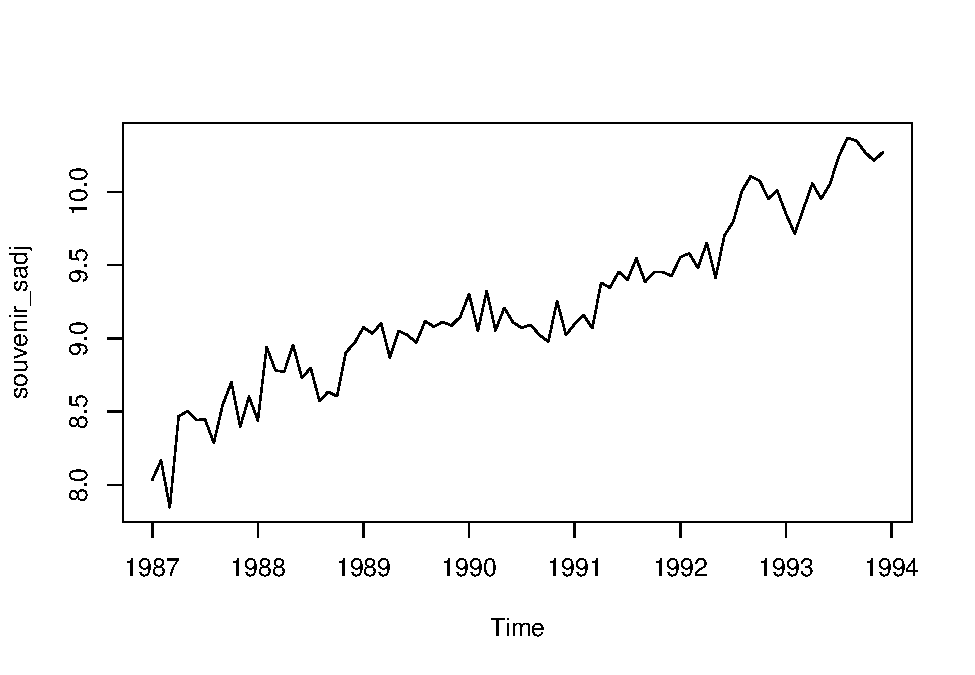
\includegraphics{dv_files/figure-latex/unnamed-chunk-31-1.pdf}

A recap of what we've done so far:

\begin{itemize}
\tightlist
\item
  Creating our ggplot graphics object through \texttt{ggplot()}\\
\item
  We specify 2 arguments in our call to ggplot; It's helpful to note
  that any argument we pass into \texttt{ggplot()} will be used as
  global options for the plot, i.e.~they apply to all layers we add onto
  that graphics object\\
\item
  For the second argument we use the \texttt{aes()} function, allowing
  us to map variables from our \texttt{gempa} data to aesthetic
  properties of the plot (in our case we map them to the x and y axis)\\
\item
  We tell ggplot how we want the graphic objects to be represented by
  adding (through the ``+'' operator) our geom layer. Since we added
  \texttt{geom\_point}, this is equivalent to adding a layer of
  scatterplot to represent our x and y variables
\end{itemize}

As we familiarize ourselves with this system, we will learn to use other
functions to obtain a more precise control over the construction of our
plot. This could be natively \texttt{ggplot} constructs such as scales,
legends, geoms and thematic elements or this could be additional
constructs that work with \texttt{ggplot} through the use of third-party
packages. In the following example, we're adding
\texttt{background\_image} to our original plot (\texttt{g}) before
adding \texttt{geom\_point} on top of the background image layer.
Finally, we add the labels for our title and caption using the
\texttt{labs} function:

\begin{Shaded}
\begin{Highlighting}[]
\KeywordTok{library}\NormalTok{(png)}
\NormalTok{jak <-}\StringTok{ }\NormalTok{png}\OperatorTok{::}\KeywordTok{readPNG}\NormalTok{(}\StringTok{'jakarta.png'}\NormalTok{)}
\NormalTok{g }\OperatorTok{+}
\StringTok{  }\KeywordTok{background_image}\NormalTok{(jak)}\OperatorTok{+}
\StringTok{  }\KeywordTok{geom_point}\NormalTok{(}\DataTypeTok{size=}\NormalTok{gempa}\OperatorTok{$}\NormalTok{size, }\DataTypeTok{alpha =} \FloatTok{0.6}\NormalTok{, }\DataTypeTok{col=}\StringTok{"red2"}\NormalTok{)}\OperatorTok{+}
\StringTok{  }\KeywordTok{labs}\NormalTok{(}\DataTypeTok{title=}\StringTok{"Disaster Impact Zone, Invasion Area 2018"}\NormalTok{, }\DataTypeTok{caption=}\StringTok{"source: Jakarta Distaster Relief"}\NormalTok{)}
\end{Highlighting}
\end{Shaded}

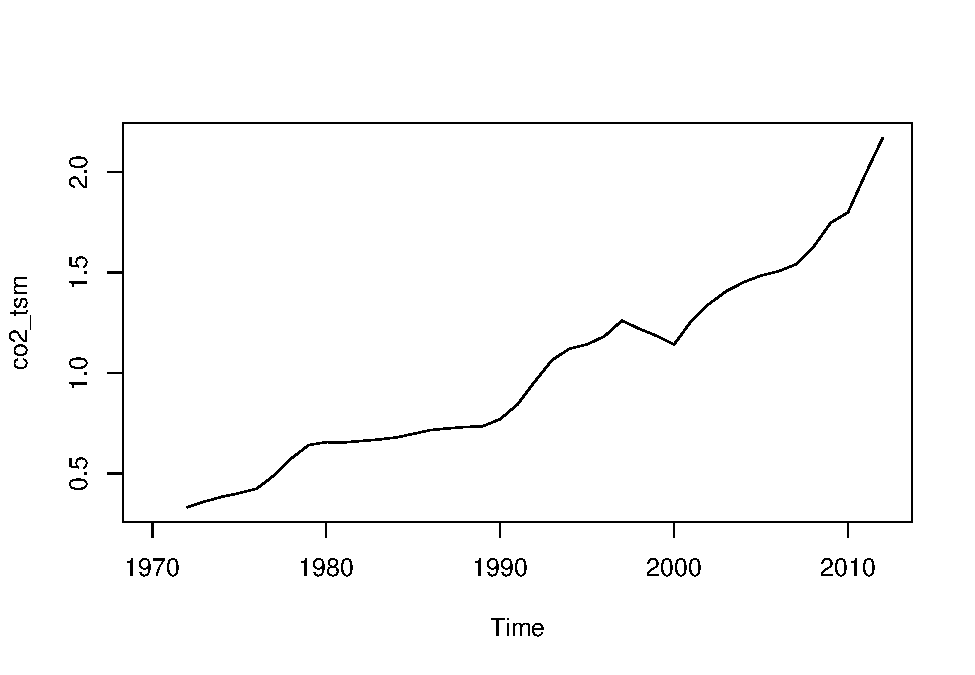
\includegraphics{dv_files/figure-latex/unnamed-chunk-32-1.pdf}

Because of this design philosophy in ggplot, it presents a learning
curve that is beginner-friendly and mostly logical. I said
beginner-friendly, because as we will see later, all we need to do is to
master the starting steps first and not worry about polishing. And with
starting steps, this means:\\
- 1: \texttt{ggplot()} with \texttt{data} and aesthetics mapping
(\texttt{aes}) - 2: Add to (1) a single \texttt{geom} layer

\hypertarget{the-state-of-trending-videos}{%
\subsection{The State of Trending
Videos}\label{the-state-of-trending-videos}}

\hypertarget{hands-on-ggplot-simple-exploratory-analysis}{%
\subsubsection{Hands-on ggplot: Simple Exploratory
Analysis}\label{hands-on-ggplot-simple-exploratory-analysis}}

Let's apply what we've learned above to create a simple plot. We will
use \texttt{vids.ags} as the data, and map our x, y, and size aesthetics
to the \texttt{category\_id}, \texttt{dislikes} and comment-per-view
respectively.

\begin{Shaded}
\begin{Highlighting}[]
\KeywordTok{ggplot}\NormalTok{(}\DataTypeTok{data =}\NormalTok{ vids.ags, }\KeywordTok{aes}\NormalTok{(}\DataTypeTok{x=}\NormalTok{category_id, }\DataTypeTok{y=}\NormalTok{dislikes, }\DataTypeTok{size=}\NormalTok{comment_count}\OperatorTok{/}\NormalTok{views))}\OperatorTok{+}
\StringTok{  }\KeywordTok{geom_jitter}\NormalTok{()}
\end{Highlighting}
\end{Shaded}

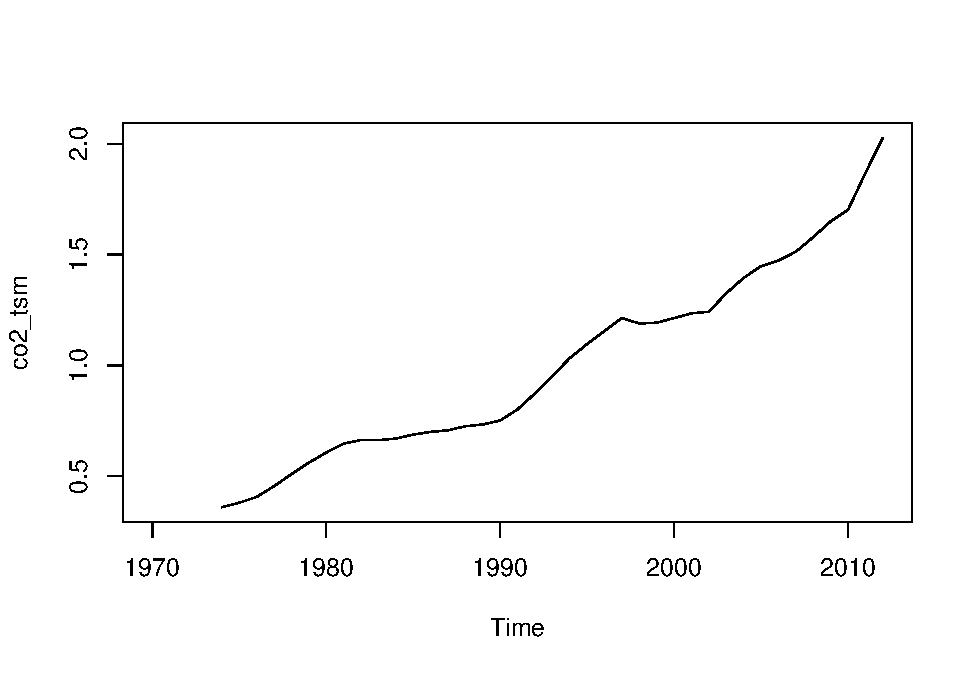
\includegraphics{dv_files/figure-latex/unnamed-chunk-33-1.pdf}

Mostly, I'm copy-and-pasting the code from earlier chunks and then
adding ggplot2 elements onto the plot layer-by-layer. Here I mapped the
color of my jitter points to the day of week for each of these videos. I
also added a \texttt{theme} component to specify the position of my
legend:

\begin{Shaded}
\begin{Highlighting}[]
\KeywordTok{ggplot}\NormalTok{(}\DataTypeTok{data =}\NormalTok{ vids.ags, }\KeywordTok{aes}\NormalTok{(}\DataTypeTok{x=}\NormalTok{category_id, }\DataTypeTok{y=}\NormalTok{dislikes, }\DataTypeTok{size=}\NormalTok{comment_count}\OperatorTok{/}\NormalTok{views))}\OperatorTok{+}
\StringTok{  }\KeywordTok{geom_jitter}\NormalTok{(}\KeywordTok{aes}\NormalTok{(}\DataTypeTok{col=}\NormalTok{publish_wday))}\OperatorTok{+}
\StringTok{  }\KeywordTok{theme}\NormalTok{(}\DataTypeTok{legend.position =} \StringTok{"none"}\NormalTok{)}
\end{Highlighting}
\end{Shaded}

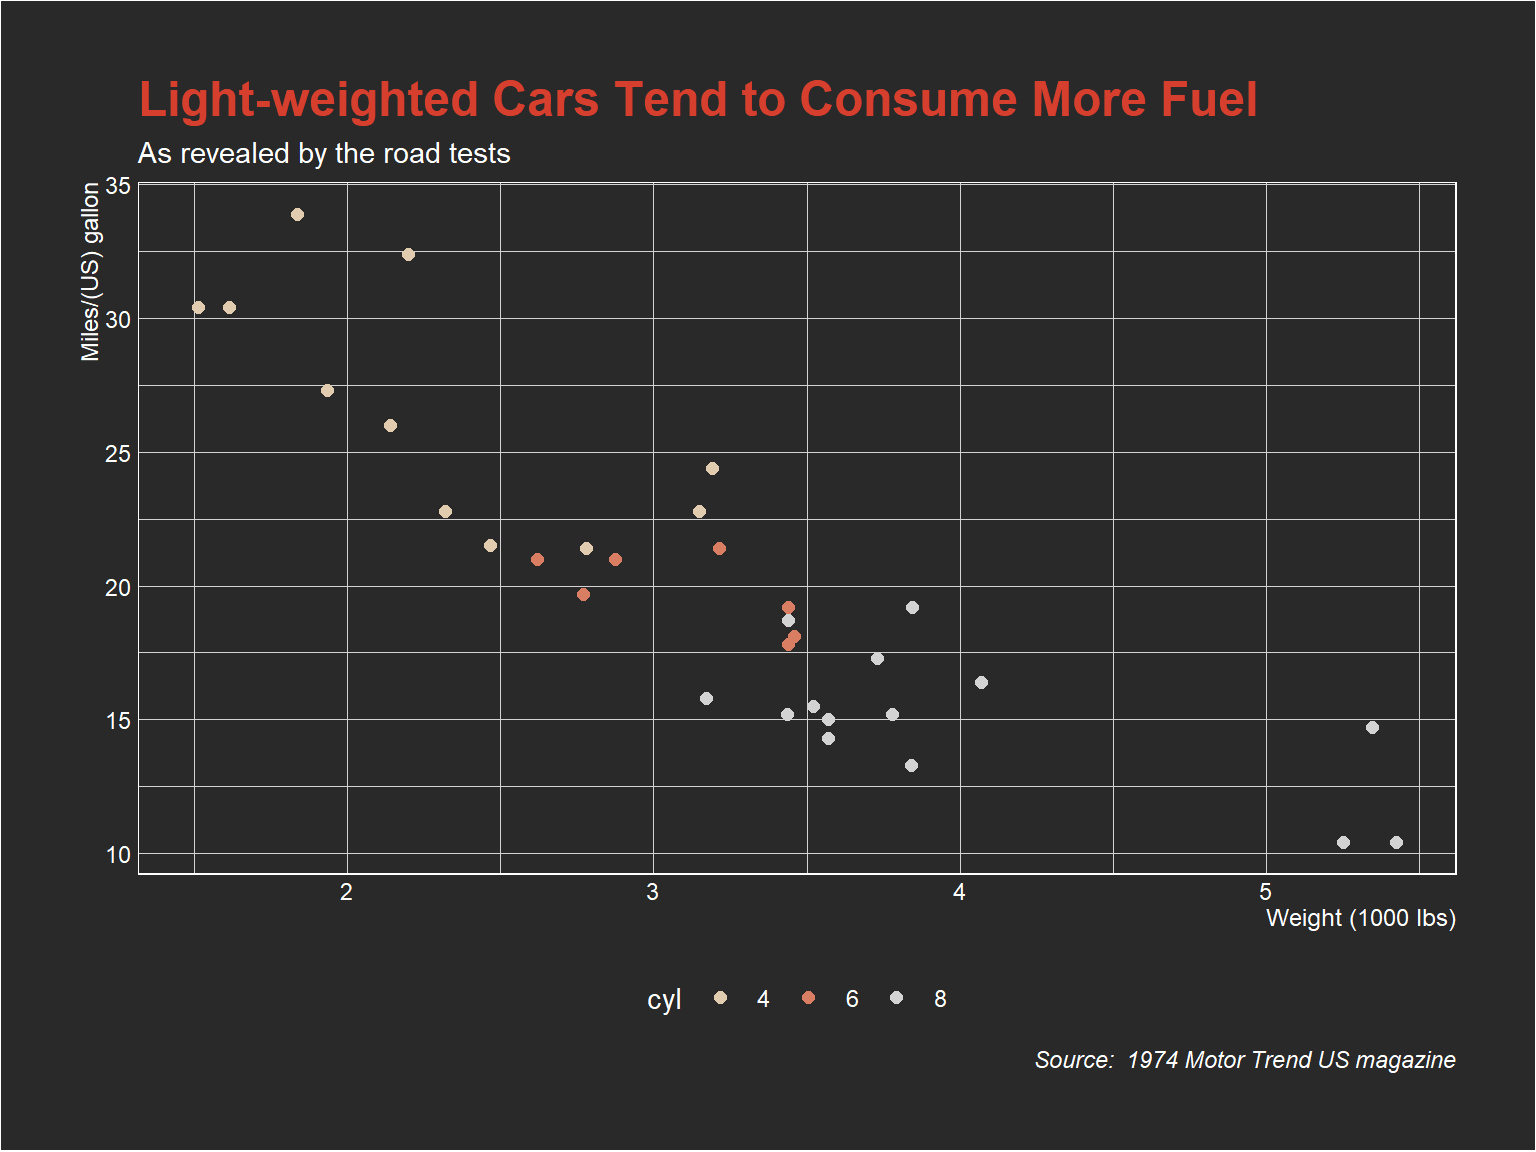
\includegraphics{dv_files/figure-latex/unnamed-chunk-34-1.pdf}

I hope you're getting the pattern now, but just to drive home the point,
let's copy the code above and add one more layer:
\texttt{geom\_boxplot()}. I want the jitter points to be above the
boxplot, so I'll add the elements in that order such that the last item
will be on the top-most:

\begin{Shaded}
\begin{Highlighting}[]
\KeywordTok{ggplot}\NormalTok{(}\DataTypeTok{data =}\NormalTok{ vids.ags, }\KeywordTok{aes}\NormalTok{(}\DataTypeTok{x=}\NormalTok{category_id, }\DataTypeTok{y=}\NormalTok{dislikes, }\DataTypeTok{size=}\NormalTok{comment_count}\OperatorTok{/}\NormalTok{views))}\OperatorTok{+}
\StringTok{  }\KeywordTok{geom_boxplot}\NormalTok{()}\OperatorTok{+}
\StringTok{  }\KeywordTok{geom_jitter}\NormalTok{(}\KeywordTok{aes}\NormalTok{(}\DataTypeTok{col=}\NormalTok{publish_wday))}\OperatorTok{+}
\StringTok{  }\KeywordTok{theme}\NormalTok{(}\DataTypeTok{legend.position =} \StringTok{"none"}\NormalTok{)}
\end{Highlighting}
\end{Shaded}

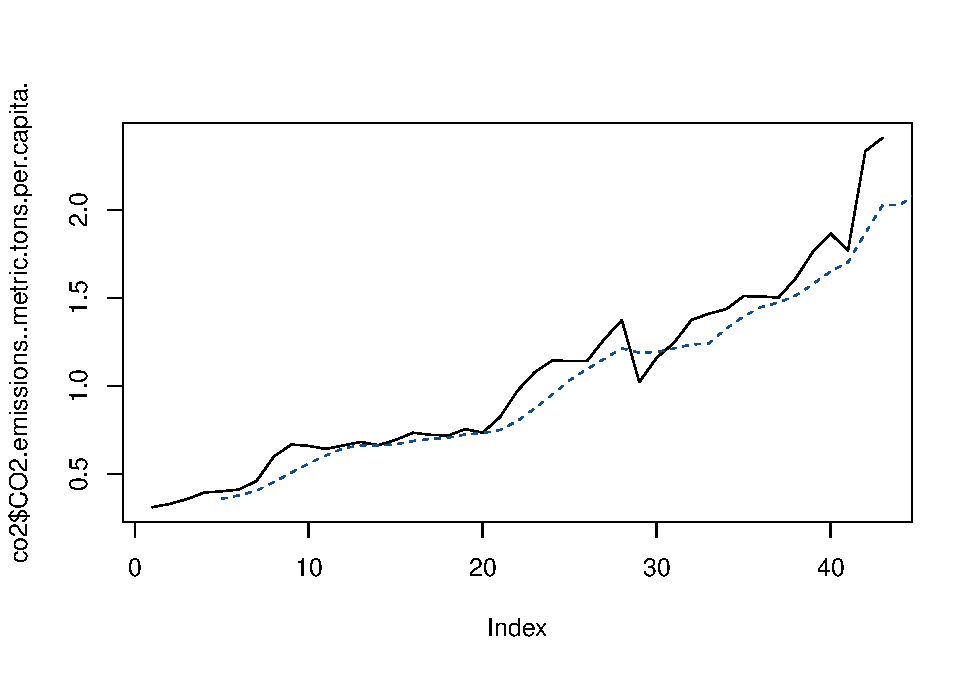
\includegraphics{dv_files/figure-latex/unnamed-chunk-35-1.pdf}

\textbf{Dive Deeper: Give our plot a main title and caption:}

Recall that we can use \texttt{labs()} to change the labels on our plot
and we did just that earlier when we gave our plot a main title and
caption. Copy (or re-write) the code above, and gave them an appropriate
title and caption. Your code should look something like this:

\begin{Shaded}
\begin{Highlighting}[]
\CommentTok{### Copy and Paste or Finish the following pseudo-code}

\CommentTok{## psuedo-code}
\CommentTok{## ggplot() +}
\CommentTok{##   geom_boxplot() +}
\CommentTok{##   geom_jitter()+}
\CommentTok{##   theme() +}
\CommentTok{##   labs(title="Dislikes to View Comparison", subtitle="Youtube Trending Data, 2018", x="Video Category",       y="Dislikes/View", caption="Made by Carl Gauss, 28 Jan 2018")}

\CommentTok{### End of Exercise}
\end{Highlighting}
\end{Shaded}

Hopefully that was a fun introduction to ggplot!

Now let's start thinking about a more useful application of plotting.
Imagine you're working with the insights and business intelligence team
at a media firm, and were asked to produce a report that illustrates the
most prolific producers of trending videos in recent weeks.

Since we're concerned about the quantity of videos (talking about being
\emph{prolific!}) we will create another subset of the full dataframe,
but take only the channels that have at least 10 videos being trending!

\begin{Shaded}
\begin{Highlighting}[]
\NormalTok{temp1 <-}\StringTok{ }\KeywordTok{as.data.frame}\NormalTok{(}\KeywordTok{table}\NormalTok{(vids.u}\OperatorTok{$}\NormalTok{channel_title))}
\NormalTok{temp1 <-}\StringTok{ }\NormalTok{temp1[temp1}\OperatorTok{$}\NormalTok{Freq }\OperatorTok{>=}\StringTok{ }\DecValTok{10}\NormalTok{,]}
\NormalTok{temp1 <-}\StringTok{ }\NormalTok{temp1[}\KeywordTok{order}\NormalTok{(temp1}\OperatorTok{$}\NormalTok{Freq, }\DataTypeTok{decreasing =}\NormalTok{ T), ]}
\KeywordTok{head}\NormalTok{(temp1)}
\end{Highlighting}
\end{Shaded}

\begin{verbatim}
##                                        Var1 Freq
## 1020                             Refinery29   31
## 1227 The Tonight Show Starring Jimmy Fallon   30
## 1355                                    Vox   29
## 1242                           TheEllenShow   28
## 882                                 Netflix   27
## 890                                     NFL   25
\end{verbatim}

\texttt{temp1} is a dataframe with two variables, and contain a list of
channels that have at least 10 videos being trending in the observation
period. Let's create a column chart (\texttt{geom\_col}). The category
names can be displayed horizontally by placing it on the \emph{x-axis}
while the frequency is placed on the \emph{y-axis}. That makes it easier
for the user to read and identify the videos that are more prolific than
others in producing trending videos:

\begin{Shaded}
\begin{Highlighting}[]
\KeywordTok{ggplot}\NormalTok{(temp1, }\KeywordTok{aes}\NormalTok{(}\DataTypeTok{x=}\NormalTok{Freq, }\DataTypeTok{y=}\NormalTok{Var1))}\OperatorTok{+}
\StringTok{  }\KeywordTok{geom_col}\NormalTok{()}
\end{Highlighting}
\end{Shaded}

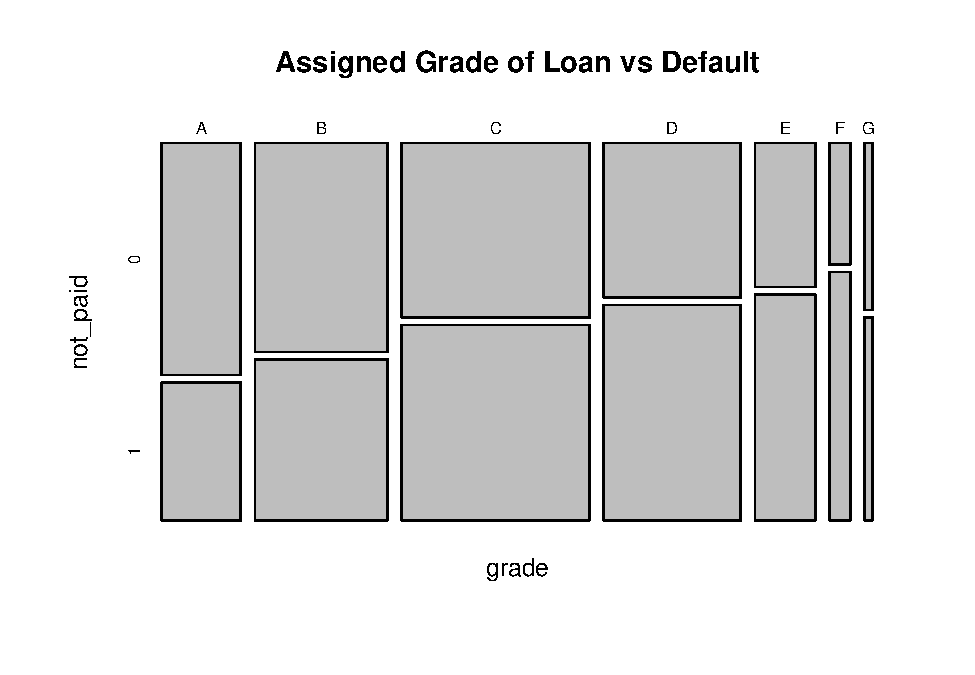
\includegraphics{dv_files/figure-latex/unnamed-chunk-38-1.pdf}

If flipping the coordinates (swapping x and y axis) isn't an option,
then another approach is to rotate the axis-text for x by 90 degree.
This is done with the following code:

\begin{Shaded}
\begin{Highlighting}[]
\KeywordTok{ggplot}\NormalTok{(temp1, }\KeywordTok{aes}\NormalTok{(}\DataTypeTok{x=}\NormalTok{Var1, }\DataTypeTok{y=}\NormalTok{Freq))}\OperatorTok{+}
\StringTok{  }\KeywordTok{geom_col}\NormalTok{()}\OperatorTok{+}
\StringTok{  }\KeywordTok{theme}\NormalTok{(}\DataTypeTok{axis.text.x =} \KeywordTok{element_text}\NormalTok{(}\DataTypeTok{angle =} \DecValTok{90}\NormalTok{, }\DataTypeTok{hjust =} \DecValTok{1}\NormalTok{))}
\end{Highlighting}
\end{Shaded}

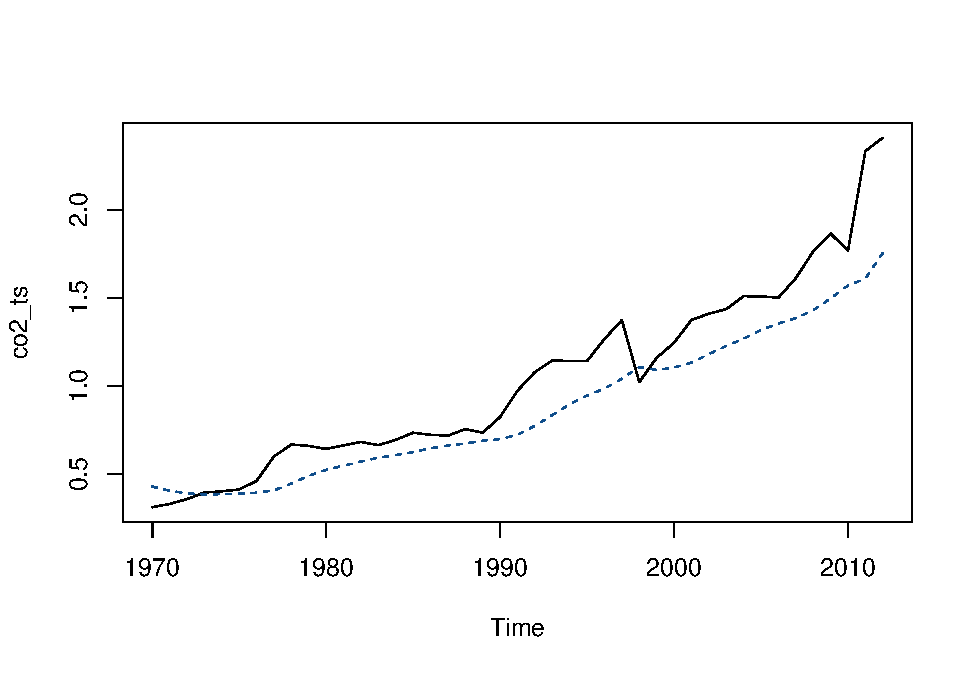
\includegraphics{dv_files/figure-latex/unnamed-chunk-39-1.pdf}

To maximize the time you spent writing code, let's hop into another Dive
Deeper challenger. This time we'll create a dataframe with two
variables: first is the \texttt{category\_id} and second being the mean
(average) of dislikes by each of these category. Using what we've
learned in Programming for Data Science we create this dataframe using
\texttt{aggregate()}

Here's the code:

\begin{Shaded}
\begin{Highlighting}[]
\NormalTok{temp2 <-}\StringTok{ }\KeywordTok{aggregate.data.frame}\NormalTok{(vids.u}\OperatorTok{$}\NormalTok{dislikes, }\DataTypeTok{by=}\KeywordTok{list}\NormalTok{(vids.u}\OperatorTok{$}\NormalTok{category_id), mean)}
\KeywordTok{head}\NormalTok{(temp2)}
\end{Highlighting}
\end{Shaded}

\begin{verbatim}
##              Group.1         x
## 1 Autos and Vehicles  155.1220
## 2             Comedy  863.9414
## 3          Education  363.7477
## 4      Entertainment 2303.7745
## 5 Film and Animation  572.9079
## 6             Gaming 1473.9667
\end{verbatim}

\textbf{Dive Deeper}: Can you use \texttt{geom\_col} to create a column
chart that plots the amount of average likes by category? Refer to
earlier exercises if you need to. Add a \texttt{labs()} component to
label the x- and y-axis appropriately as a bonus.

\begin{Shaded}
\begin{Highlighting}[]
\CommentTok{# Write your codes here}
\end{Highlighting}
\end{Shaded}

Now what is important here is that the above did not account for the
views each of these category has, and so before jumping into any
conclusion it's paramount we think with clarity and purpose the
``biases'' our plot or statistics may show. Perhaps a better idea is to
have our dislikes ``adjusted for'' the views, so it is more
representative of the true events!

Just to freshen things up, we'll shift the focus from \textbf{video
categories} to \textbf{video producers} for this next exercise. We're
now creating a subset of the dataframe that measures the
dislikes-to-views and comment count, but group it on a channel /
producer level instead of a categorical level. We'll make sure to take
only observations with a non-zero value for the comment count:

\begin{Shaded}
\begin{Highlighting}[]
\NormalTok{temp3 <-}\StringTok{ }\KeywordTok{aggregate.data.frame}\NormalTok{(}\KeywordTok{list}\NormalTok{(}\DataTypeTok{dislikeratio =}\NormalTok{ vids.u}\OperatorTok{$}\NormalTok{dislikes}\OperatorTok{/}\NormalTok{vids.u}\OperatorTok{$}\NormalTok{views, }\DataTypeTok{comment =}\NormalTok{ vids.u}\OperatorTok{$}\NormalTok{comment_count), }\DataTypeTok{by=}\KeywordTok{list}\NormalTok{(vids.u}\OperatorTok{$}\NormalTok{channel_title), mean)}
\NormalTok{temp3 <-}\StringTok{ }\NormalTok{temp3[}\KeywordTok{order}\NormalTok{(temp3}\OperatorTok{$}\NormalTok{dislikeratio, }\DataTypeTok{decreasing =}\NormalTok{ T), ]}
\NormalTok{temp3 <-}\StringTok{ }\NormalTok{temp3[temp3}\OperatorTok{$}\NormalTok{comment }\OperatorTok{!=}\StringTok{ }\DecValTok{0}\NormalTok{, ]}
\KeywordTok{head}\NormalTok{(temp3)}
\end{Highlighting}
\end{Shaded}

\begin{verbatim}
##               Group.1 dislikeratio  comment
## 293      Daily Caller   0.19153148  28013.0
## 779    MatthewSantoro   0.04705022   7484.0
## 724  Logan Paul Vlogs   0.02926234 434266.0
## 462     Gigi Gorgeous   0.02879144   4477.0
## 905            NJ.com   0.02736082    147.0
## 1235  The White House   0.02150297   2870.5
\end{verbatim}

With the newly created dataframe \texttt{temp3}, let's try and create a
plot similar to the dot plot we see in an earlier exercise. For now,
don't worry about coloring the points or labels and just use a fixed
color. However, have the size of each point correspond to the comment
count of the videos.

The solution code is here:

\begin{Shaded}
\begin{Highlighting}[]
\KeywordTok{ggplot}\NormalTok{(temp3[}\DecValTok{1}\OperatorTok{:}\DecValTok{20}\NormalTok{,], }\KeywordTok{aes}\NormalTok{(}\DataTypeTok{x=}\NormalTok{dislikeratio, }\DataTypeTok{y=}\NormalTok{Group}\FloatTok{.1}\NormalTok{))}\OperatorTok{+}
\StringTok{  }\KeywordTok{geom_point}\NormalTok{(}\KeywordTok{aes}\NormalTok{(}\DataTypeTok{size=}\NormalTok{comment), }\DataTypeTok{color=}\StringTok{"goldenrod4"}\NormalTok{,}\DataTypeTok{show.legend =}\NormalTok{ F)}\OperatorTok{+}
\StringTok{  }\KeywordTok{scale_size}\NormalTok{(}\DataTypeTok{range=}\KeywordTok{c}\NormalTok{(}\DecValTok{1}\NormalTok{,}\DecValTok{11}\NormalTok{))}
\end{Highlighting}
\end{Shaded}

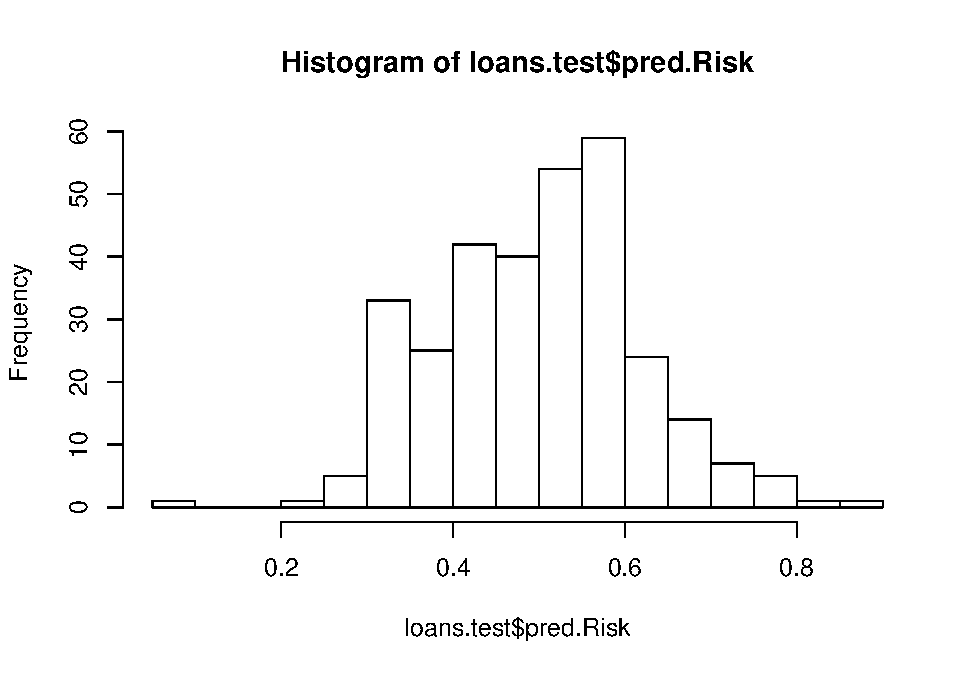
\includegraphics{dv_files/figure-latex/unnamed-chunk-43-1.pdf}

Notice for example that among the top 20 most disliked trending videos,
\textbf{Daily Channel} is credited with the most disastrous dislike
ratio - close to 18 dislikes per 100 view! Note also that channels such
as \textbf{Logan Paul Vlogs} and to a smaller extent \textbf{FaZe Rug}
have videos that garnered a fair bit of presumably hate / unkind
comments, more so than the rest of the crop. It is important to be
reminded that here we're looking at 20 of the most disliked videos in
our entire dataset!

We can swap the axis to any other geoms as well to get a better
visualization. Such flexbility clearly has much to offer when the data
we want to visualize is relatively large, making the right arrangement
of the plot's element especially important. Let's see an example below:

\begin{Shaded}
\begin{Highlighting}[]
\KeywordTok{ggplot}\NormalTok{(vids.u[vids.u}\OperatorTok{$}\NormalTok{ratings_disabled }\OperatorTok{==}\StringTok{ }\NormalTok{F, ], }\KeywordTok{aes}\NormalTok{(}\DataTypeTok{x=}\NormalTok{likes}\OperatorTok{/}\NormalTok{views, }\DataTypeTok{y=}\NormalTok{category_id))}\OperatorTok{+}
\StringTok{  }\KeywordTok{geom_boxplot}\NormalTok{(}\DataTypeTok{show.legend =}\NormalTok{ F, }\DataTypeTok{color=}\StringTok{"goldenrod4"}\NormalTok{)}
\end{Highlighting}
\end{Shaded}

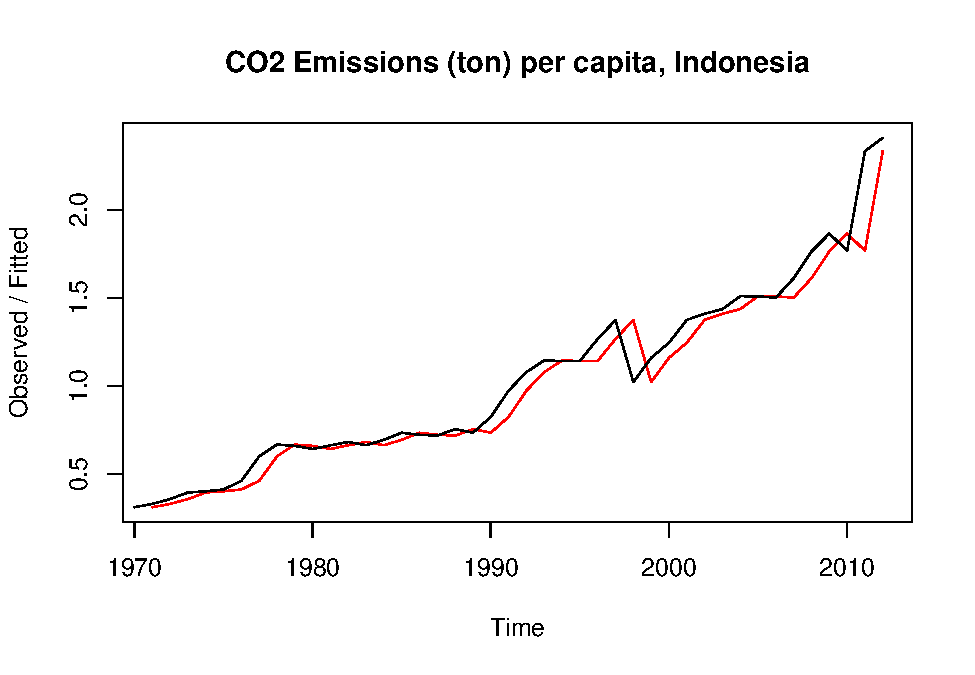
\includegraphics{dv_files/figure-latex/unnamed-chunk-44-1.pdf}

A potentially noisy plot, with some clever arrangement, can be made
simple and effortless with ggplot. Spend a couple of minutes before
hopping into the next section to understand, and practice, what you've
learned so far. Hopefully you've seen enough to be convinced of the
merits and advantages of this plotting system.

\hypertarget{hands-on-ggplot-multivariate-plots}{%
\subsubsection{Hands-on ggplot: Multivariate
Plots}\label{hands-on-ggplot-multivariate-plots}}

To take things up a notch, let's see how we can apply what we've learned
to create multivariate plots, or plots designed to reveal the
relationship among multiple variables, which in turn help us examine the
underlying patterns between pairs of variables.

To facilitate our tasks, I'm introducing a \texttt{package} called
\texttt{tidyr}, which allow us to reshape a data frame between ``wide''
(measurement spread across horizontally) and ``long'' (measurement
collected vertically). The principle of wide and long format can be
illustrated with the following figures.

\begin{center}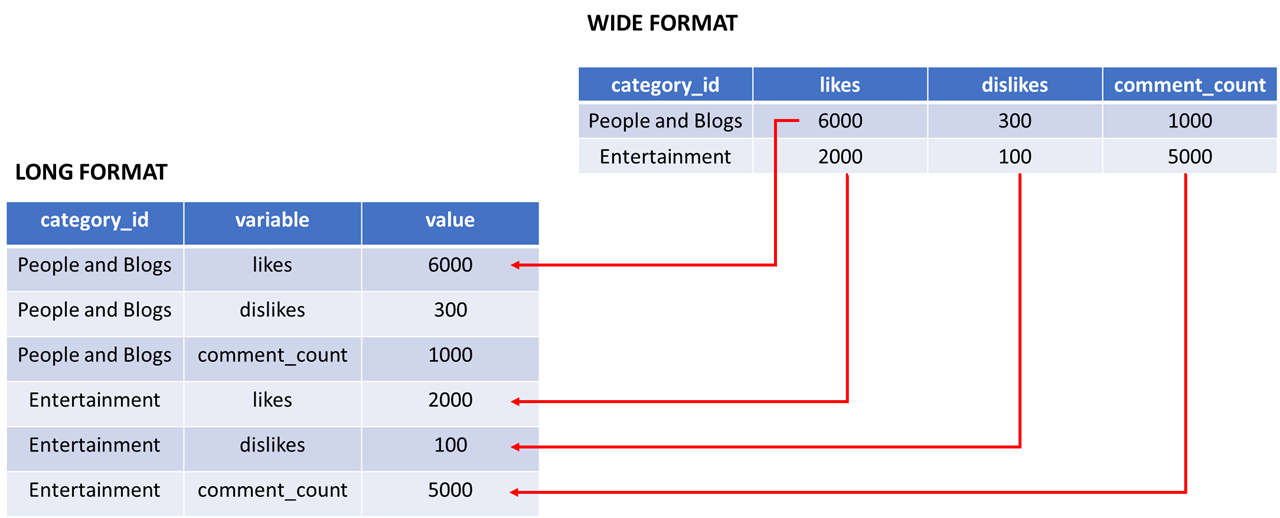
\includegraphics[width=1\linewidth]{assets/long_wide} \end{center}

In the following code, I'm reshaping the \texttt{vids.u} dataframe from
a wide one to a long one, with \texttt{category\_id} being the ID and
measurements being \texttt{likes}, \texttt{dislikes} and
\texttt{comment\_count}:

\begin{Shaded}
\begin{Highlighting}[]
\KeywordTok{library}\NormalTok{(tidyr)}
\CommentTok{# 4,8,7,9 pointing to category_id, likes, dislikes, comment_count}
\NormalTok{vids.select <-}\StringTok{ }\NormalTok{vids.u[vids.u}\OperatorTok{$}\NormalTok{comments_disabled }\OperatorTok{==}\StringTok{ }\NormalTok{F,}
                      \KeywordTok{c}\NormalTok{(}\DecValTok{4}\NormalTok{,}\DecValTok{7}\NormalTok{,}\DecValTok{8}\NormalTok{,}\DecValTok{9}\NormalTok{)]}

\CommentTok{# reshape data from wide format to long format}
\NormalTok{vids.m <-}\StringTok{ }\KeywordTok{pivot_longer}\NormalTok{(}\DataTypeTok{data =}\NormalTok{ vids.select, }
                       \DataTypeTok{cols =} \OperatorTok{-}\NormalTok{category_id, }
                       \DataTypeTok{names_to =} \StringTok{"variable"}\NormalTok{, }
                       \DataTypeTok{values_to =} \StringTok{"value"}\NormalTok{)}

\KeywordTok{rbind}\NormalTok{(}\KeywordTok{head}\NormalTok{(vids.m), }\KeywordTok{tail}\NormalTok{(vids.m))}
\end{Highlighting}
\end{Shaded}

\begin{verbatim}
## # A tibble: 12 x 3
##    category_id      variable      value
##    <fct>            <chr>         <dbl>
##  1 People and Blogs likes         57527
##  2 People and Blogs dislikes       2966
##  3 People and Blogs comment_count 15954
##  4 Entertainment    likes         97185
##  5 Entertainment    dislikes       6146
##  6 Entertainment    comment_count 12703
##  7 Sports           likes           136
##  8 Sports           dislikes          5
##  9 Sports           comment_count    16
## 10 Entertainment    likes          3246
## 11 Entertainment    dislikes         28
## 12 Entertainment    comment_count   386
\end{verbatim}

And using the melted dataframe, we can now create \texttt{ggplot}. As a
start, we'll create a column plot and visualize the \texttt{value} of
each \texttt{variable} in each of the \texttt{category\_id}. We map the
color of each bars to \texttt{variable\_id} using \texttt{fill} like the
following:

\begin{Shaded}
\begin{Highlighting}[]
\KeywordTok{ggplot}\NormalTok{(vids.m, }\KeywordTok{aes}\NormalTok{(}\DataTypeTok{x=}\NormalTok{value, }\DataTypeTok{y=}\NormalTok{category_id))}\OperatorTok{+}
\StringTok{  }\KeywordTok{geom_col}\NormalTok{(}\DataTypeTok{position=}\StringTok{"dodge"}\NormalTok{, }\KeywordTok{aes}\NormalTok{(}\DataTypeTok{fill=}\NormalTok{variable))}
\end{Highlighting}
\end{Shaded}

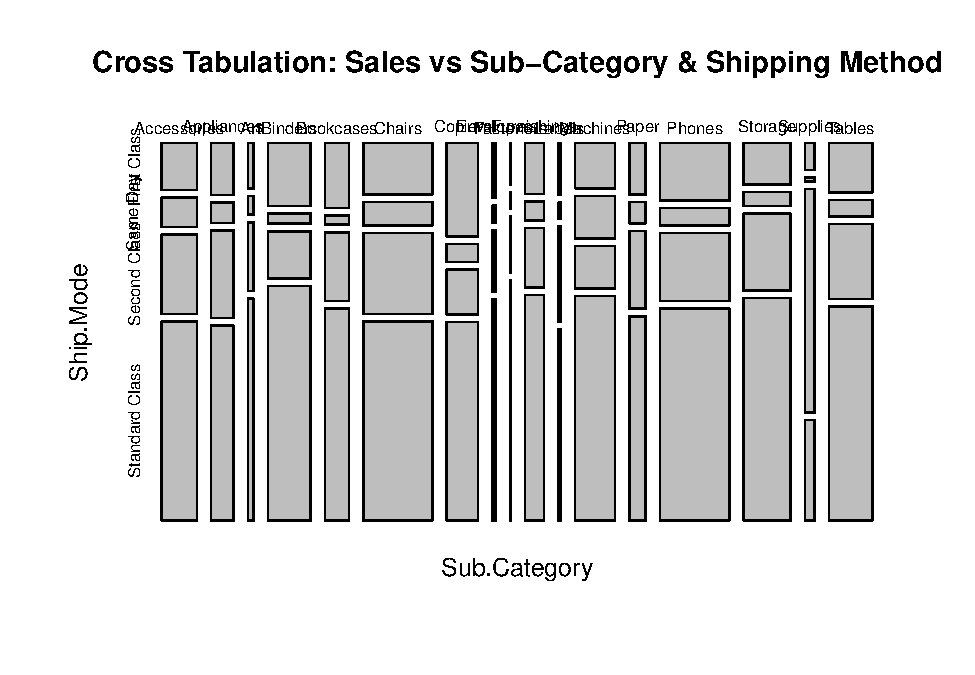
\includegraphics{dv_files/figure-latex/unnamed-chunk-47-1.pdf}

If you have wanted a stacked bar plot instead of side-by-side bar plots,
all we need to do is to substitute the \texttt{position="dodge"}
parameter with \texttt{position="stack"}. Try that in the code chunk
above and see the resulting plot adjust to that!

Using the same technique above, we'll create another melted dataframe
using only videos that have more dislikes than likes
(\texttt{dislikes\ \textgreater{}=\ likes}) with the exclusion of any
video that have their ratings disabled:

\begin{Shaded}
\begin{Highlighting}[]
\CommentTok{# 4,8,7,9 pointing to category_id, likes, dislikes, comment_count}
\NormalTok{vids.select2 <-}\StringTok{ }\NormalTok{vids.u[vids.u}\OperatorTok{$}\NormalTok{dislikes }\OperatorTok{>=}\StringTok{ }\NormalTok{vids.u}\OperatorTok{$}\NormalTok{likes }\OperatorTok{&}\StringTok{ }\NormalTok{vids.u}\OperatorTok{$}\NormalTok{ratings_disabled }\OperatorTok{==}\StringTok{ }\NormalTok{F, }
                       \KeywordTok{c}\NormalTok{(}\DecValTok{4}\NormalTok{,}\DecValTok{7}\NormalTok{,}\DecValTok{8}\NormalTok{,}\DecValTok{9}\NormalTok{)]}

\NormalTok{vids.hate <-}\StringTok{ }\KeywordTok{pivot_longer}\NormalTok{(}\DataTypeTok{data =}\NormalTok{ vids.select2, }
                          \DataTypeTok{cols =} \OperatorTok{-}\NormalTok{category_id, }
                          \DataTypeTok{names_to =} \StringTok{"variable"}\NormalTok{, }
                          \DataTypeTok{values_to =} \StringTok{"value"}\NormalTok{)}
\KeywordTok{head}\NormalTok{(vids.hate)}
\end{Highlighting}
\end{Shaded}

\begin{verbatim}
## # A tibble: 6 x 3
##   category_id variable      value
##   <fct>       <chr>         <dbl>
## 1 Music       likes         15186
## 2 Music       dislikes      15448
## 3 Music       comment_count  7484
## 4 Sports      likes          2017
## 5 Sports      dislikes       2425
## 6 Sports      comment_count  1447
\end{verbatim}

And let's create a dodge-type bar plot just like above:

\begin{Shaded}
\begin{Highlighting}[]
\KeywordTok{ggplot}\NormalTok{(vids.hate, }\KeywordTok{aes}\NormalTok{(}\DataTypeTok{x=}\NormalTok{value, }\DataTypeTok{y=}\NormalTok{category_id))}\OperatorTok{+}
\StringTok{  }\KeywordTok{geom_col}\NormalTok{(}\DataTypeTok{position=}\StringTok{"dodge"}\NormalTok{, }\KeywordTok{aes}\NormalTok{(}\DataTypeTok{fill=}\NormalTok{variable))}
\end{Highlighting}
\end{Shaded}

\includegraphics{dv_files/figure-latex/unnamed-chunk-49-1.pdf}

From the plot above, the trending videos that were disliked by YouTube
users seem to have come from the \textbf{People and Blogs} and
\textbf{News and Politics} categories in no small amount. This may
indicate a category-level pattern, or such skew may be attributed to
only a handful of ``bad actors''. To investigate further, let's apply
the techniques we've learned above but this time we'll melt the
dataframe by \texttt{channel\_title} instead of categories:

\begin{Shaded}
\begin{Highlighting}[]
\NormalTok{vids.hate2 <-}\StringTok{ }\KeywordTok{pivot_longer}\NormalTok{(}\DataTypeTok{data =}\NormalTok{ vids.u[vids.u}\OperatorTok{$}\NormalTok{dislikes }\OperatorTok{>=}\StringTok{ }\DecValTok{10000} \OperatorTok{&}
\StringTok{                                           }\NormalTok{vids.u}\OperatorTok{$}\NormalTok{dislikes}\OperatorTok{*}\DecValTok{2} \OperatorTok{>=}\StringTok{ }\NormalTok{vids.u}\OperatorTok{$}\NormalTok{likes }\OperatorTok{&}\StringTok{ }
\StringTok{                                           }\NormalTok{vids.u}\OperatorTok{$}\NormalTok{ratings_disabled }\OperatorTok{==}\StringTok{ }\NormalTok{F, }
                                         \KeywordTok{c}\NormalTok{(}\DecValTok{3}\NormalTok{,}\DecValTok{7}\NormalTok{,}\DecValTok{8}\NormalTok{,}\DecValTok{9}\NormalTok{)], }
                          \DataTypeTok{cols =} \OperatorTok{-}\NormalTok{channel_title, }
                          \DataTypeTok{names_to =} \StringTok{"variable"}\NormalTok{, }
                          \DataTypeTok{values_to =} \StringTok{"value"}\NormalTok{)}

\KeywordTok{head}\NormalTok{(vids.hate2[}\KeywordTok{order}\NormalTok{(vids.hate2}\OperatorTok{$}\NormalTok{channel_title),])}
\end{Highlighting}
\end{Shaded}

\begin{verbatim}
## # A tibble: 6 x 3
##   channel_title                  variable       value
##   <chr>                          <chr>          <dbl>
## 1 Daily Caller                   likes           9100
## 2 Daily Caller                   dislikes      218841
## 3 Daily Caller                   comment_count  28013
## 4 Full Frontal with Samantha Bee likes          11383
## 5 Full Frontal with Samantha Bee dislikes       12122
## 6 Full Frontal with Samantha Bee comment_count   4289
\end{verbatim}

And creating our \texttt{ggplot()}:

\begin{Shaded}
\begin{Highlighting}[]
\KeywordTok{ggplot}\NormalTok{(vids.hate2, }\KeywordTok{aes}\NormalTok{(}\DataTypeTok{x=}\NormalTok{channel_title, }\DataTypeTok{y=}\NormalTok{value))}\OperatorTok{+}
\StringTok{  }\KeywordTok{geom_col}\NormalTok{(}\KeywordTok{aes}\NormalTok{(}\DataTypeTok{fill=}\NormalTok{variable))}\OperatorTok{+}
\StringTok{  }\KeywordTok{theme}\NormalTok{(}\DataTypeTok{axis.text.x =} \KeywordTok{element_text}\NormalTok{(}\DataTypeTok{angle =} \DecValTok{90}\NormalTok{, }\DataTypeTok{hjust =} \DecValTok{1}\NormalTok{))}
\end{Highlighting}
\end{Shaded}

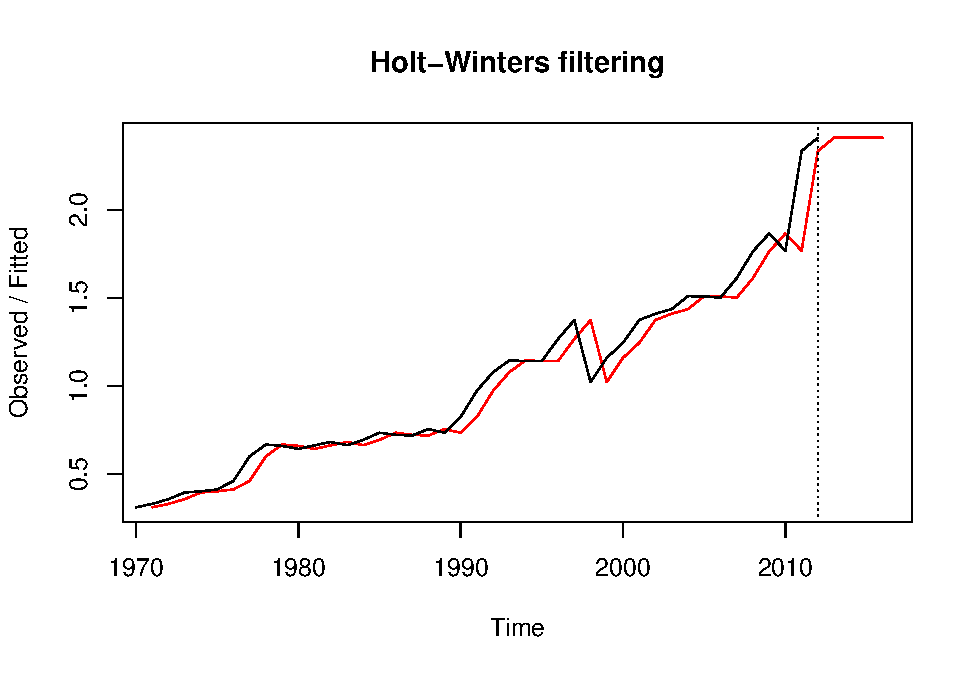
\includegraphics{dv_files/figure-latex/unnamed-chunk-51-1.pdf}

Sure enough, we see that there are three peculiar cases from ``Daily
Caller'', ``Logan Paul Vlogs'' and to a lesser extent ``Washington
Post''.

Daily Caller is a far-right news and opinion website that posted a
controversial and potentially offensive video titled ``PSA from Chairman
of the FCC Ajit Pai''. In this video, the FCC Chairman dismisses
concerns over net neutrality while dancing around in a Santa suit to
``Harlem Shake'' and swinging a lightsaber. Logan Paul, back in December
2017 published a disturbing video titled ``Found Dead Body in Forest''
that featured actual footage of what appears to be a dead body when he
and his friends ventured into Aokigahara (known also as the Suicide
Forest) and subsequently a video titled ``so sorry''.

Washington Post's ``The FCC repeals its net neutrality rules'' was third
on the most disliked trending videos, and it is actually a 3-hour long
live stream in which federal regulators vote to allow Internet providers
to speed up service for some apps and websites --- and block or slow
down others. The decision is considered highly unpopular.

Let's pick out the Trending videos published by Logan Paul and create a
new variable that calculates the likes-to-dislikes ratio:

\begin{Shaded}
\begin{Highlighting}[]
\NormalTok{vids.logan <-}\StringTok{ }\NormalTok{vids[vids}\OperatorTok{$}\NormalTok{channel_title }\OperatorTok{==}\StringTok{ "Logan Paul Vlogs"}\NormalTok{,]}
\NormalTok{vids.logan}\OperatorTok{$}\NormalTok{sentiment <-}\StringTok{ }\NormalTok{(vids.logan}\OperatorTok{$}\NormalTok{likes}\OperatorTok{/}\NormalTok{vids.logan}\OperatorTok{$}\NormalTok{dislikes)}\OperatorTok{*}\DecValTok{100}
\end{Highlighting}
\end{Shaded}

The following is one way to compare the sentiments. There is nothing new
in the following code and you should be able to fully understand what
the code is doing:

\begin{Shaded}
\begin{Highlighting}[]
\KeywordTok{ggplot}\NormalTok{(vids.logan, }\KeywordTok{aes}\NormalTok{(}\DataTypeTok{x=}\NormalTok{trending_date, }\DataTypeTok{y=}\NormalTok{sentiment, }\DataTypeTok{color=}\NormalTok{title))}\OperatorTok{+}
\StringTok{  }\KeywordTok{geom_point}\NormalTok{(}\KeywordTok{aes}\NormalTok{(}\DataTypeTok{size=}\NormalTok{views))}\OperatorTok{+}
\StringTok{  }\KeywordTok{guides}\NormalTok{(}\DataTypeTok{size=}\NormalTok{F)}\OperatorTok{+}
\StringTok{  }\KeywordTok{theme}\NormalTok{(}\DataTypeTok{legend.position =} \StringTok{"bottom"}\NormalTok{)}
\end{Highlighting}
\end{Shaded}

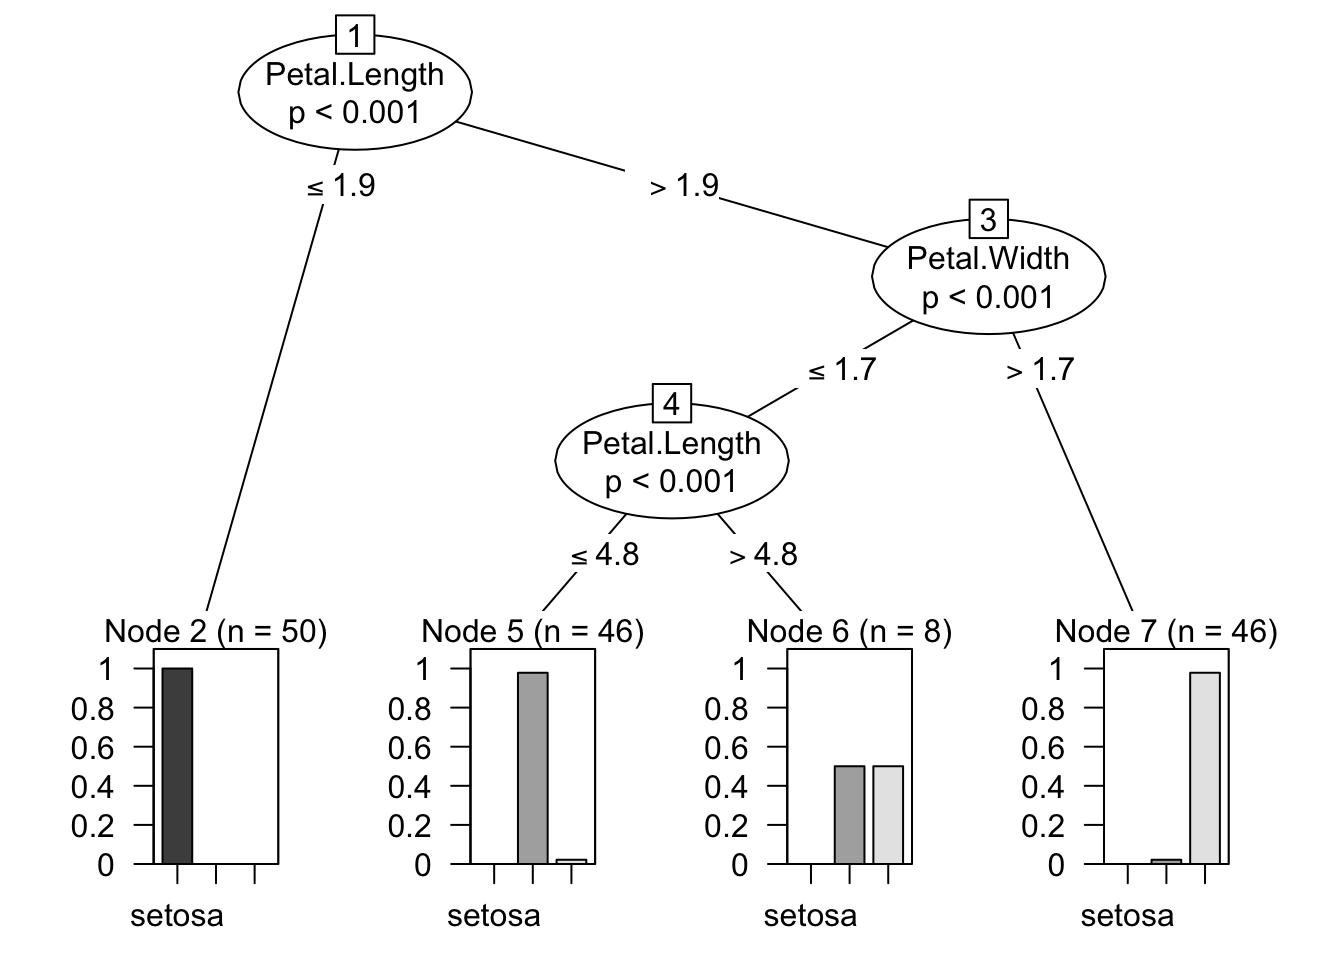
\includegraphics{dv_files/figure-latex/unnamed-chunk-53-1.pdf} Observe
that we're using the size to represent views, but that wasn't very
obvious to our readers. We can add a legend or accompanying annotation
to explain that, but as we'll see in the coming exercises there are
better way to represent these data.

While the y-axis still represents the sentiment, we will add a layer of
\texttt{geom\_label} to label the movie names instead. A similar
function would have been \texttt{geom\_text} but since we're practically
labelling our points, I've opted for the \texttt{geom\_label} instead.
Here, we're looking at the trending videos from Universal Pictures
during that period.

\begin{Shaded}
\begin{Highlighting}[]
\KeywordTok{ggplot}\NormalTok{(vids.u[vids.u}\OperatorTok{$}\NormalTok{channel_title }\OperatorTok{==}\StringTok{ "Universal Pictures"}\NormalTok{, ], }\KeywordTok{aes}\NormalTok{(}\DataTypeTok{x=}\NormalTok{trending_date, }\DataTypeTok{y=}\NormalTok{likes}\OperatorTok{/}\NormalTok{dislikes, }\DataTypeTok{color=}\NormalTok{comment_count, }\DataTypeTok{size=}\NormalTok{views))}\OperatorTok{+}
\StringTok{  }\KeywordTok{geom_point}\NormalTok{(}\KeywordTok{aes}\NormalTok{(}\DataTypeTok{size=}\NormalTok{views),}\DataTypeTok{show.legend =}\NormalTok{ F)}\OperatorTok{+}
\StringTok{  }\KeywordTok{geom_label}\NormalTok{(}\KeywordTok{aes}\NormalTok{(}\DataTypeTok{label=}\NormalTok{title), }\DataTypeTok{nudge_y =} \DecValTok{1}\NormalTok{, }\DataTypeTok{label.size =} \DecValTok{1}\NormalTok{, }\DataTypeTok{hjust=}\StringTok{"inward"}\NormalTok{, }\DataTypeTok{size=}\DecValTok{3}\NormalTok{)}\OperatorTok{+}
\StringTok{  }\KeywordTok{scale_color_gradient}\NormalTok{(}\DataTypeTok{low=}\StringTok{"green4"}\NormalTok{, }\DataTypeTok{high=}\StringTok{"green2"}\NormalTok{)}\OperatorTok{+}
\StringTok{  }\KeywordTok{theme}\NormalTok{(}\DataTypeTok{legend.position =} \StringTok{"none"}\NormalTok{)}
\end{Highlighting}
\end{Shaded}

\includegraphics{dv_files/figure-latex/unnamed-chunk-54-1.pdf} Now this
plot communicates about the same level of information with more
directness (no need for the use of legends), and it's immediately clear
that \textbf{Jurassic World: Fallen Kingdom - Official Trailer {[}HD{]}}
is the most-viewed, as well as the most-loved (highest likes to dislikes
ratio) among them.

\hypertarget{hands-on-ggplot-multiple-groups-of-data}{%
\subsubsection{Hands-on ggplot: Multiple groups of
data}\label{hands-on-ggplot-multiple-groups-of-data}}

To add a bit of diversity in our exercise, we'll now subset from our
original data any videos produced by the channel \textbf{Tasty} and we
will also compute the mean on each of these videos across the different
days it was featured on - these are represented as \texttt{tasty} and
\texttt{tasty.agg} respectively:

\begin{Shaded}
\begin{Highlighting}[]
\NormalTok{tasty <-}\StringTok{ }\NormalTok{vids[vids}\OperatorTok{$}\NormalTok{channel_title }\OperatorTok{==}\StringTok{ "Tasty"}\NormalTok{, ]}
\NormalTok{tasty.agg <-}\StringTok{ }\KeywordTok{aggregate.data.frame}\NormalTok{(tasty}\OperatorTok{$}\NormalTok{views, }\DataTypeTok{by =} \KeywordTok{list}\NormalTok{(tasty}\OperatorTok{$}\NormalTok{title), mean)}
\KeywordTok{names}\NormalTok{(tasty.agg) <-}\StringTok{ }\KeywordTok{c}\NormalTok{(}\StringTok{"title"}\NormalTok{, }\StringTok{"mean"}\NormalTok{)}
\NormalTok{tasty.agg}
\end{Highlighting}
\end{Shaded}

\begin{verbatim}
##                                                            title     mean
## 1 5 Desserts To Share with your BFF at Max Brenner Chocolate Bar 298912.2
## 2                               Homemade Vs. Store-bought: Pasta 620141.7
## 3                     Restaurant Vs. Homemade Chicken Parm Pizza 494174.7
## 4                     The Best Ever Vegan Chocolate Chip Cookies 248983.6
## 5                                         Ultimate Bacon Recipes 413071.2
\end{verbatim}

Sometimes we want to visualize relationships between variables in
multiple subsets of the data - in these situations a particularly
elegant solution is to have the plots appearing in panels defined in our
plot construction process. These types of plots are called facet plots
and is an incredible feature of ggplot. Let's see how we can take
advantage of that!

Here we're creating a plot using the \texttt{tasty} dataset, first by
creating the columns and then adding a second layer of points, and
finally horizontal lines \texttt{geom\_hline} (an equivalent for
vertical line would be \texttt{geom\_vline}) for each mean in our
\texttt{tasty.agg} dataframe. By passing in \texttt{data=tasty.agg}, it
overrides the initial data (\texttt{tasty}) allowing us to add plot
elements using aesthetic from a different dataframe. Because we have 5
rows of means, we would expect 5 dashed lines (\texttt{linetype=2}).

\begin{Shaded}
\begin{Highlighting}[]
\NormalTok{g1 <-}\StringTok{ }\KeywordTok{ggplot}\NormalTok{(tasty, }\KeywordTok{aes}\NormalTok{(}\DataTypeTok{x=}\NormalTok{trending_date, }\DataTypeTok{y=}\NormalTok{views))}\OperatorTok{+}
\StringTok{  }\KeywordTok{geom_col}\NormalTok{()}\OperatorTok{+}
\StringTok{  }\KeywordTok{geom_point}\NormalTok{(}\KeywordTok{aes}\NormalTok{(}\DataTypeTok{col=}\NormalTok{likes}\OperatorTok{/}\NormalTok{dislikes))}\OperatorTok{+}
\StringTok{  }\KeywordTok{geom_hline}\NormalTok{(}\DataTypeTok{data=}\NormalTok{tasty.agg, }\KeywordTok{aes}\NormalTok{(}\DataTypeTok{yintercept=}\NormalTok{mean),}\DataTypeTok{linetype=}\DecValTok{2}\NormalTok{)}

\NormalTok{g1}
\end{Highlighting}
\end{Shaded}

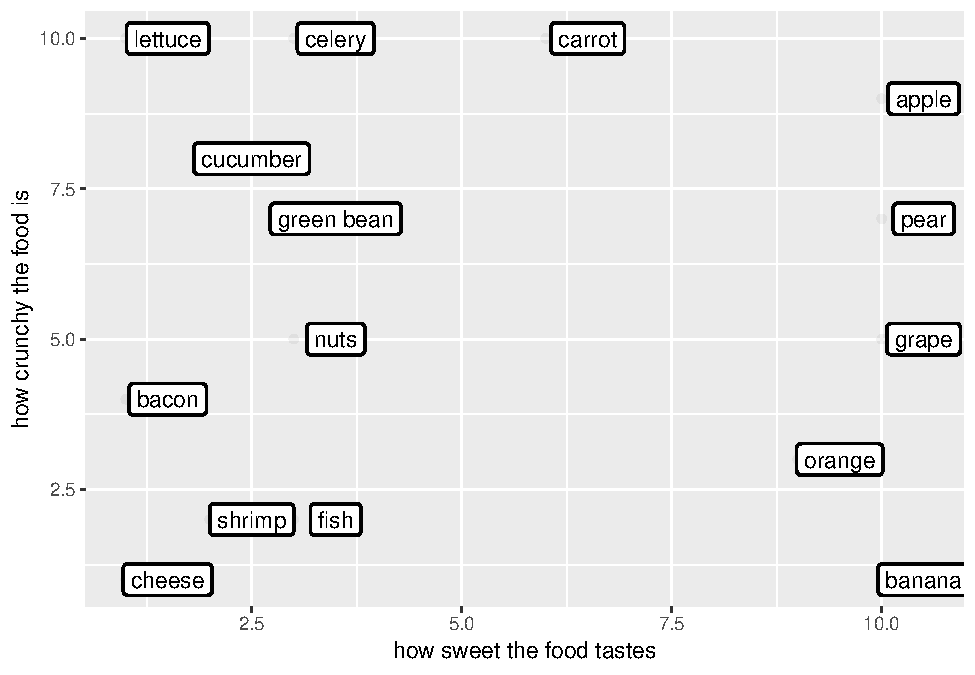
\includegraphics{dv_files/figure-latex/unnamed-chunk-56-1.pdf}

It isn't a bad start, but it may have been a better design decision to
break the plot up into panels by each video so we can have a better
observation of each video's trend. This could be established using
\texttt{facet\_wrap()}. \texttt{facet\_wrap} wraps our plots into a
multirow panel of plots. Here we'll specify the number of columns to be
2 using \texttt{ncol=2}:

\begin{Shaded}
\begin{Highlighting}[]
\NormalTok{g1 }\OperatorTok{+}
\StringTok{  }\KeywordTok{geom_line}\NormalTok{(}\DataTypeTok{col=}\StringTok{"black"}\NormalTok{)}\OperatorTok{+}
\StringTok{  }\KeywordTok{facet_wrap}\NormalTok{(}\OperatorTok{~}\KeywordTok{as.factor}\NormalTok{(title), }\DataTypeTok{ncol=}\DecValTok{2}\NormalTok{)}\OperatorTok{+}
\StringTok{  }\KeywordTok{scale_color_gradient}\NormalTok{(}\DataTypeTok{low=}\StringTok{"yellow"}\NormalTok{, }\DataTypeTok{high=}\StringTok{"green2"}\NormalTok{)}\OperatorTok{+}
\StringTok{  }\KeywordTok{theme}\NormalTok{(}\DataTypeTok{legend.position =} \StringTok{"none"}\NormalTok{, }
        \DataTypeTok{strip.text=}\KeywordTok{element_text}\NormalTok{(}\DataTypeTok{size=}\DecValTok{7}\NormalTok{))}
\end{Highlighting}
\end{Shaded}

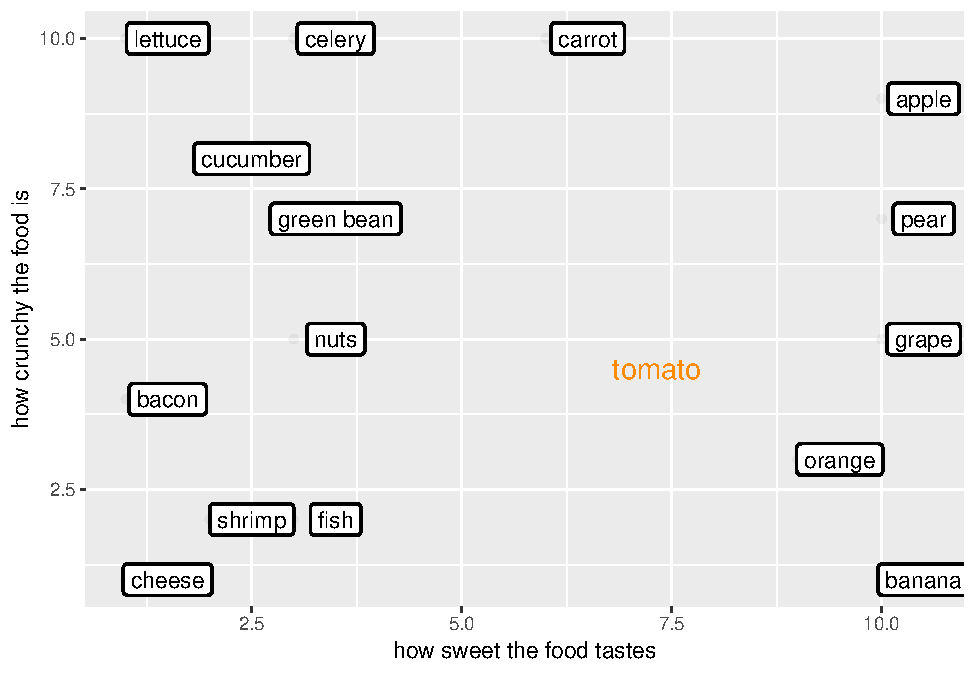
\includegraphics{dv_files/figure-latex/unnamed-chunk-57-1.pdf}

In a similar way to \texttt{facet\_wrap}, we can use
\texttt{facet\_grid} to specify which variables are used to split our
plots along the rows and columns. If we want the row to be the day of
the week and columns to represent each category, we could achieve that
by adding
\texttt{facet\_grid(publish\_wday\textasciitilde{}as.factor(category\_id))}:

\begin{Shaded}
\begin{Highlighting}[]
\KeywordTok{ggplot}\NormalTok{(}\DataTypeTok{data=}\NormalTok{vids.agt, }\KeywordTok{aes}\NormalTok{(}\DataTypeTok{x=}\NormalTok{timetotrend, }\DataTypeTok{y=}\NormalTok{likes}\OperatorTok{/}\NormalTok{views))}\OperatorTok{+}
\StringTok{  }\KeywordTok{geom_jitter}\NormalTok{(}\KeywordTok{aes}\NormalTok{(}\DataTypeTok{size=}\NormalTok{views, }\DataTypeTok{col=}\NormalTok{likes))}\OperatorTok{+}
\StringTok{  }\KeywordTok{facet_grid}\NormalTok{(publish_wday}\OperatorTok{~}\KeywordTok{as.factor}\NormalTok{(category_id))}\OperatorTok{+}
\StringTok{  }\KeywordTok{scale_size}\NormalTok{(}\DataTypeTok{range=}\KeywordTok{c}\NormalTok{(}\DecValTok{1}\NormalTok{,}\DecValTok{3}\NormalTok{))}\OperatorTok{+}
\StringTok{  }\KeywordTok{theme}\NormalTok{(}\DataTypeTok{legend.position =} \StringTok{"none"}\NormalTok{, }
        \DataTypeTok{strip.text=}\KeywordTok{element_text}\NormalTok{(}\DataTypeTok{size=}\DecValTok{5}\NormalTok{))}
\end{Highlighting}
\end{Shaded}

\includegraphics{dv_files/figure-latex/unnamed-chunk-58-1.pdf}

\textbf{Dive Deeper: Using facet\_grids or facet\_wraps on Vox media}
Imagine working with Vox media and tasked to produce a visualization
using data of their trending videos in past recent weeks. Use either
\texttt{facet\_wrap} or \texttt{facet\_grid} in your visualization.

\begin{Shaded}
\begin{Highlighting}[]
\NormalTok{vids.vox <-}\StringTok{ }\NormalTok{vids.u[vids.u}\OperatorTok{$}\NormalTok{channel_title }\OperatorTok{==}\StringTok{ "Vox"}\NormalTok{, ]}
\NormalTok{vids.vox}\OperatorTok{$}\NormalTok{sentiment <-}\StringTok{ }\NormalTok{vids.vox}\OperatorTok{$}\NormalTok{likes}\OperatorTok{/}\NormalTok{vids.vox}\OperatorTok{$}\NormalTok{dislikes}
\NormalTok{vids.vox}\OperatorTok{$}\NormalTok{title <-}\StringTok{ }\KeywordTok{as.factor}\NormalTok{(vids.vox}\OperatorTok{$}\NormalTok{title)}
\KeywordTok{head}\NormalTok{(vids.vox)}
\end{Highlighting}
\end{Shaded}

\begin{verbatim}
##      trending_date                                                    title
## 10      2017-11-14 Why the rise of the robots won\x89۪t mean the end of work
## 411     2017-11-16    The all-American fruit you've probably never heard of
## 614     2017-11-17                                      Walking while black
## 807     2017-11-18          The environmental cost of free two-day shipping
## 1003    2017-11-19                 The military coup in Zimbabwe, explained
## 1419    2017-11-21 How job surveillance is transforming trucking in America
##      channel_title       category_id        publish_time  views likes dislikes
## 10             Vox News and Politics 2017-11-13 13:45:16 256426 12654     1363
## 411            Vox News and Politics 2017-11-15 11:30:00 533940 12633      597
## 614            Vox News and Politics 2017-11-16 12:55:39 505886 23207     5375
## 807            Vox News and Politics 2017-11-17 13:00:12 366048 14742     1308
## 1003           Vox News and Politics 2017-11-18 16:09:31 396346 11277      499
## 1419           Vox News and Politics 2017-11-20 13:01:34 455289 14025      441
##      comment_count comments_disabled ratings_disabled video_error_or_removed
## 10            2368             FALSE            FALSE                  FALSE
## 411           1828             FALSE            FALSE                  FALSE
## 614           7030             FALSE            FALSE                  FALSE
## 807           1948             FALSE            FALSE                  FALSE
## 1003          2140             FALSE            FALSE                  FALSE
## 1419          2340             FALSE            FALSE                  FALSE
##      publish_hour publish_when publish_wday timetotrend sentiment
## 10             13   8am to 3pm       Monday           1  9.283933
## 411            11   8am to 3pm    Wednesday           1 21.160804
## 614            12   8am to 3pm     Thursday           1  4.317581
## 807            13   8am to 3pm       Friday           1 11.270642
## 1003           16  3pm to 12am     Saturday           1 22.599198
## 1419           13   8am to 3pm       Monday           1 31.802721
\end{verbatim}

\begin{Shaded}
\begin{Highlighting}[]
\CommentTok{### Write your answer here and execute the code to produce your visualization}

\CommentTok{# -- Scroll up to refer to earlier code and copy / paste any if you like }
\CommentTok{# -- Try and attempt this challenge by discussion with your neighbor if necessary but do not blindly copy his / her code and produce the work on your own!}
\end{Highlighting}
\end{Shaded}

While I'll show you a reference answer here below, I strongly recommend
you only use this as a reference upon completion of the \textbf{Dive
Deeper} exercise.

\begin{Shaded}
\begin{Highlighting}[]
\NormalTok{voxp <-}\StringTok{ }\KeywordTok{ggplot}\NormalTok{(vids.vox, }\KeywordTok{aes}\NormalTok{(}\DataTypeTok{x=}\NormalTok{trending_date, }\DataTypeTok{y=}\NormalTok{comment_count, }\DataTypeTok{color=}\NormalTok{sentiment))}\OperatorTok{+}
\StringTok{  }\CommentTok{# geom_point is a reference, geom_col or other geoms (sensible choices) would work too }
\StringTok{  }\KeywordTok{geom_point}\NormalTok{(}\KeywordTok{aes}\NormalTok{(}\DataTypeTok{size=}\NormalTok{views),}\DataTypeTok{show.legend =}\NormalTok{ F, }\DataTypeTok{alpha=}\FloatTok{0.5}\NormalTok{)}\OperatorTok{+}
\StringTok{  }\KeywordTok{scale_color_gradient}\NormalTok{(}\DataTypeTok{low=}\StringTok{"red3"}\NormalTok{, }\DataTypeTok{high=}\StringTok{"green2"}\NormalTok{)}\OperatorTok{+}
\StringTok{  }\CommentTok{# facet_wrap by publish when is a reference, any other variables (sensible choices) would work}
\StringTok{  }\KeywordTok{facet_wrap}\NormalTok{(}\OperatorTok{~}\NormalTok{publish_when, }\DataTypeTok{ncol=}\DecValTok{1}\NormalTok{)}

\NormalTok{voxp}
\end{Highlighting}
\end{Shaded}

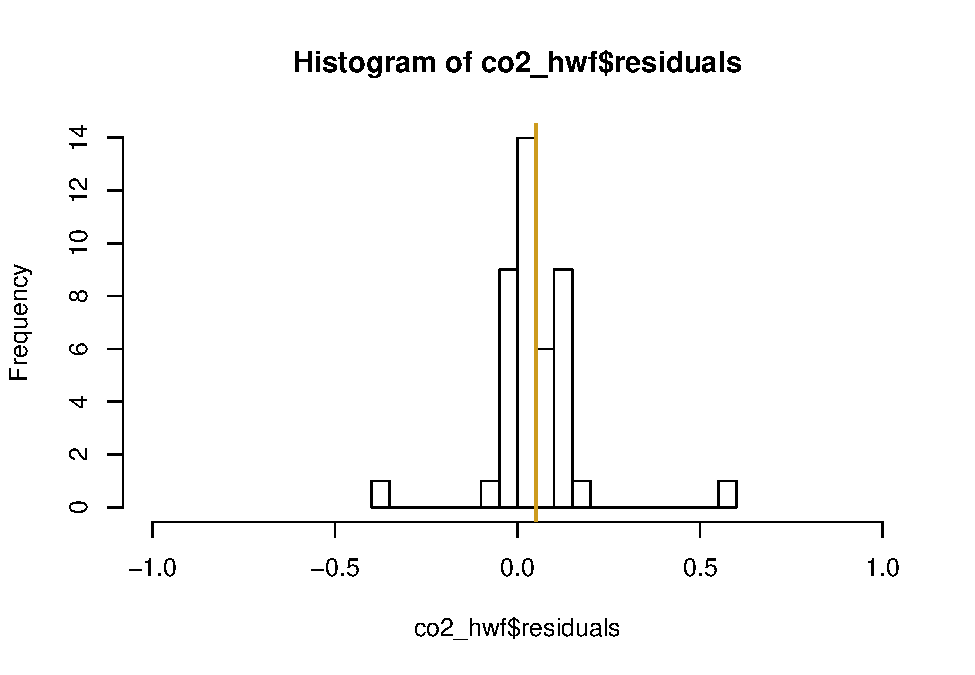
\includegraphics{dv_files/figure-latex/unnamed-chunk-61-1.pdf}

There are some pretty interesting points in the above plot. The bright
green one near ``December 01'' is an interesting video we may want to
further study, and the one that crosses 12,500 comment count is just
about as interesting. One quick fix is to replace each points with
\texttt{geom\_text} or use \texttt{geom\_label} to label them:

\begin{Shaded}
\begin{Highlighting}[]
\NormalTok{voxp }\OperatorTok{+}\StringTok{ }
\StringTok{  }\KeywordTok{geom_label}\NormalTok{(}\KeywordTok{aes}\NormalTok{(}\DataTypeTok{label=}\NormalTok{title), }\DataTypeTok{size=}\FloatTok{1.4}\NormalTok{, }\DataTypeTok{nudge_y =} \DecValTok{800}\NormalTok{) }\OperatorTok{+}
\StringTok{  }\KeywordTok{theme}\NormalTok{(}\DataTypeTok{legend.position =} \StringTok{"none"}\NormalTok{)}
\end{Highlighting}
\end{Shaded}

Notice that a lot of these labels overlapped with each other and are
generally just noisy to look at (a phenomenon sometimes called
``overplotting''). We have a few ways to fix that. First, is to only
plot points that could be potentially interesting. Second, is to have
the text or labels ``repel'' each other, creating more space between
these different points.

This can be achieved using a library called \texttt{ggrepel}:

\begin{Shaded}
\begin{Highlighting}[]
\KeywordTok{library}\NormalTok{(ggrepel)}
\NormalTok{vox.pop <-}\StringTok{ }\NormalTok{vids.vox[vids.vox}\OperatorTok{$}\NormalTok{views }\OperatorTok{>=}\StringTok{ }\DecValTok{400000} \OperatorTok{|}\StringTok{ }\NormalTok{vids.vox}\OperatorTok{$}\NormalTok{sentiment }\OperatorTok{>=}\StringTok{ }\KeywordTok{median}\NormalTok{(vids.vox}\OperatorTok{$}\NormalTok{sentiment), }\DecValTok{2}\NormalTok{]}

\NormalTok{voxp }\OperatorTok{+}\StringTok{ }
\StringTok{  }\KeywordTok{geom_label_repel}\NormalTok{(}\KeywordTok{aes}\NormalTok{(}\DataTypeTok{label=}\NormalTok{title), }\DataTypeTok{size=}\FloatTok{1.2}\NormalTok{, }\DataTypeTok{data=}\NormalTok{vids.vox[vids.vox}\OperatorTok{$}\NormalTok{title }\OperatorTok\StringTok{ }\NormalTok{vox.pop,], }\DataTypeTok{box.padding =} \FloatTok{0.4}\NormalTok{)}\OperatorTok{+}
\StringTok{  }\KeywordTok{theme}\NormalTok{(}\DataTypeTok{legend.position =} \StringTok{"none"}\NormalTok{)}
\end{Highlighting}
\end{Shaded}

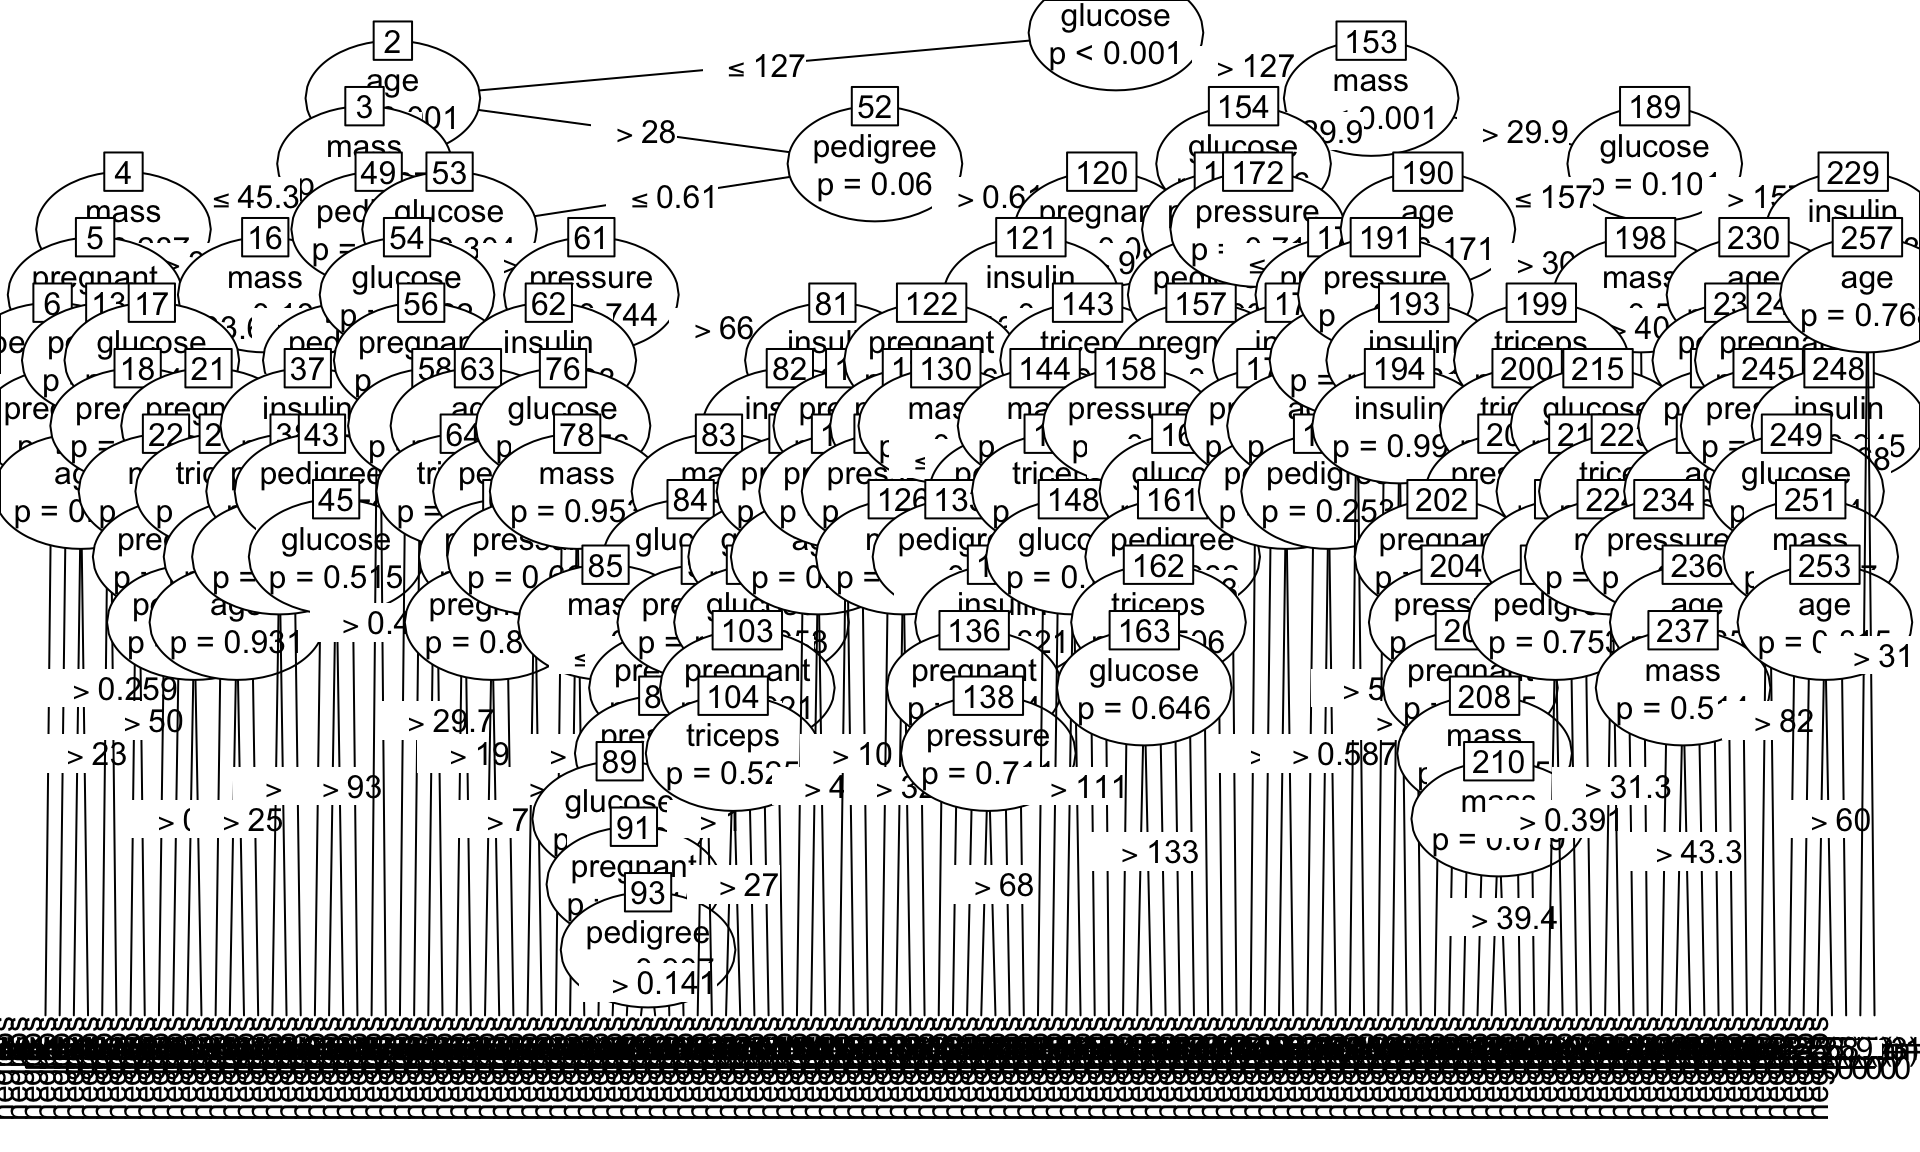
\includegraphics{dv_files/figure-latex/unnamed-chunk-63-1.pdf}

Now this result is a lot neater, and definitely more comfortable on the
eyes. We see that ``2017, in 7 minutes'' isn't at all well-liked in
terms of sentiment (more dislikes to likes ratio than many other videos
on average) even though it does seem to be trendy in every other
measures: views, indicated by the point's size; and comment counts,
indicated by it's position on the y-axis.

Topics that are trendy (lots of views, lots of comment) but unpopular do
also seem to share a thematic commonality:\\
- The real reason American health care is so expensive\\
- How Trump makes extreme things look normal\\
- The new US law, explained with cereal\\
- Walking while black\\
- The US medical system is still haunted by slavery

These 5 videos are closest to the negative end of the sentiment scale,
and the topics are sensitive or political in nature. Videos that do seem
to do very well (high approval ratings) are:\\
- How technicolor changed movies\\
- Where babies in movies come from\\
- How smart is today's artificial intelligence?\\
- Takeout creates a lot of trash. It doesn't have to\\
- Nasa's plan to save Earth from a giant asteroid

These videos seem to be scientific in nature - so this visualization do
seem to suggest a certain correlation between thematic elements and
approval ratings.

Can you discuss any other findings or propose any preliminary
observations from the plot above? How would you improve the plot above?

\hypertarget{learn-by-building-module-data-visualization}{%
\subsection{Learn-by-building Module: Data
Visualization}\label{learn-by-building-module-data-visualization}}

To help us get ready to the learn-by-building assignment, we'll walk
through a simple exercise together. There isn't any new concept being
introduced, but rather a start-to-finish recap of the data visualization
process.

First, we'll have to subset any videos within the News and Politics
category and take only the ones that have more than 10 trending videos
during the explanatory period. We run the following code and see that 6
channels / publishers satisfy that condition:

\begin{Shaded}
\begin{Highlighting}[]
\NormalTok{news <-}\StringTok{ }\NormalTok{vids.u[vids.u}\OperatorTok{$}\NormalTok{category_id }\OperatorTok{==}\StringTok{ "News and Politics"}\NormalTok{, ]}
\NormalTok{news <-}\StringTok{ }\KeywordTok{aggregate}\NormalTok{(trending_date }\OperatorTok{~}\StringTok{ }\NormalTok{channel_title, news, length)}
\NormalTok{news <-}\StringTok{ }\NormalTok{news[news}\OperatorTok{$}\NormalTok{trending_date }\OperatorTok{>}\StringTok{ }\DecValTok{10}\NormalTok{, ]}
\NormalTok{news <-}\StringTok{ }\NormalTok{news[}\KeywordTok{order}\NormalTok{(news}\OperatorTok{$}\NormalTok{trending_date, }\DataTypeTok{decreasing =}\NormalTok{ T),]}
\NormalTok{news}
\end{Highlighting}
\end{Shaded}

\begin{verbatim}
##      channel_title trending_date
## 83             Vox            29
## 30             CNN            17
## 10        BBC News            12
## 84 Washington Post            12
## 40   Guardian News            11
## 78           TODAY            11
\end{verbatim}

We can now use
\texttt{vids.u\$channel\_title\ \%in\%\ news\$channel\_title} as our
data source, indicating that we only wish to create our ggplot using
channels that are in the list of 6 news channels above. The rest of the
code is relatively straightforward:

\begin{Shaded}
\begin{Highlighting}[]
\KeywordTok{ggplot}\NormalTok{(}\DataTypeTok{data=}\NormalTok{vids.u[vids.u}\OperatorTok{$}\NormalTok{channel_title }\OperatorTok\StringTok{ }\NormalTok{news}\OperatorTok{$}\NormalTok{channel_title,], }\KeywordTok{aes}\NormalTok{(}\DataTypeTok{x=}\NormalTok{publish_time, }\DataTypeTok{y=}\NormalTok{views))}\OperatorTok{+}
\StringTok{  }\KeywordTok{geom_point}\NormalTok{(}\KeywordTok{aes}\NormalTok{(}\DataTypeTok{col=}\KeywordTok{log}\NormalTok{(likes}\OperatorTok{/}\NormalTok{dislikes), }\DataTypeTok{size=}\NormalTok{comment_count))}\OperatorTok{+}
\StringTok{  }\KeywordTok{facet_grid}\NormalTok{(publish_wday}\OperatorTok{~}\NormalTok{channel_title)}\OperatorTok{+}
\StringTok{  }\KeywordTok{scale_color_gradient}\NormalTok{(}\DataTypeTok{low=}\StringTok{"red3"}\NormalTok{, }\DataTypeTok{high=}\StringTok{"green2"}\NormalTok{)}\OperatorTok{+}
\StringTok{  }\KeywordTok{theme}\NormalTok{(}\DataTypeTok{legend.position =} \StringTok{"none"}\NormalTok{,}
        \DataTypeTok{axis.text.x =} \KeywordTok{element_text}\NormalTok{(}\DataTypeTok{angle =} \DecValTok{90}\NormalTok{, }\DataTypeTok{hjust =} \DecValTok{1}\NormalTok{))}
\end{Highlighting}
\end{Shaded}

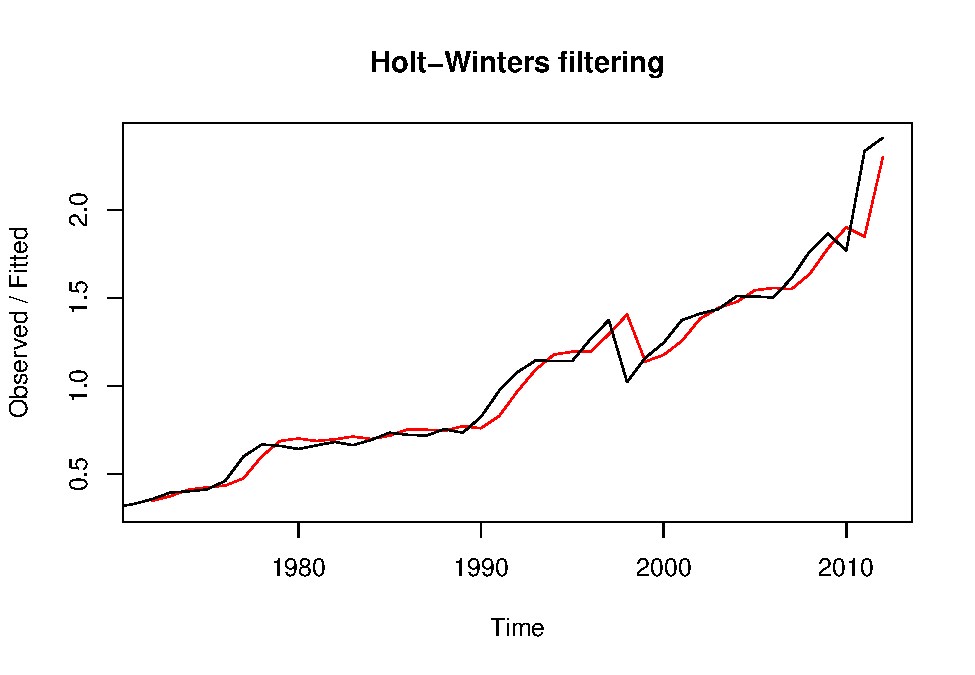
\includegraphics{dv_files/figure-latex/unnamed-chunk-65-1.pdf}

We don't always need to use a facet plot, if the information you wish to
convey doesn't require that. The following plot does not tells us the
sentiment or comment count of each video, but does enough to tell us
about each channel's representation in the trending videos.

\begin{Shaded}
\begin{Highlighting}[]
\NormalTok{news.agg <-}\StringTok{ }\NormalTok{vids.u[vids.u}\OperatorTok{$}\NormalTok{channel_title }\OperatorTok\StringTok{ }\NormalTok{news}\OperatorTok{$}\NormalTok{channel_title, ]}
\NormalTok{news.agg <-}\StringTok{ }\KeywordTok{aggregate}\NormalTok{(views }\OperatorTok{~}\StringTok{ }\NormalTok{channel_title, news.agg, mean)}
\KeywordTok{names}\NormalTok{(news.agg) <-}\StringTok{ }\KeywordTok{c}\NormalTok{(}\StringTok{"channel_title"}\NormalTok{, }\StringTok{"mean_views"}\NormalTok{)}
\NormalTok{news.agg}
\end{Highlighting}
\end{Shaded}

\begin{verbatim}
##     channel_title mean_views
## 1        BBC News   170525.0
## 2             CNN   274701.6
## 3   Guardian News   328777.5
## 4           TODAY   194893.6
## 5             Vox   517597.6
## 6 Washington Post   109853.3
\end{verbatim}

The plot:

\begin{Shaded}
\begin{Highlighting}[]
\KeywordTok{ggplot}\NormalTok{(}\DataTypeTok{data=}\NormalTok{vids.u[vids.u}\OperatorTok{$}\NormalTok{channel_title }\OperatorTok\StringTok{ }\NormalTok{news}\OperatorTok{$}\NormalTok{channel_title,], }\KeywordTok{aes}\NormalTok{(}\DataTypeTok{x=}\NormalTok{publish_time, }\DataTypeTok{y=}\NormalTok{views))}\OperatorTok{+}
\StringTok{  }\KeywordTok{geom_hline}\NormalTok{(}\DataTypeTok{data=}\NormalTok{news.agg, }\KeywordTok{aes}\NormalTok{(}\DataTypeTok{yintercept=}\NormalTok{mean_views, }\DataTypeTok{col=}\NormalTok{channel_title), }\DataTypeTok{linetype=}\DecValTok{2}\NormalTok{, }\DataTypeTok{alpha=}\FloatTok{0.8}\NormalTok{)}\OperatorTok{+}
\StringTok{  }\KeywordTok{geom_point}\NormalTok{(}\KeywordTok{aes}\NormalTok{(}\DataTypeTok{size=}\NormalTok{likes}\OperatorTok{/}\NormalTok{views, }\DataTypeTok{col=}\NormalTok{channel_title), }\DataTypeTok{stroke=}\DecValTok{1}\NormalTok{, }\DataTypeTok{alpha=}\FloatTok{0.85}\NormalTok{)}\OperatorTok{+}
\StringTok{  }\KeywordTok{guides}\NormalTok{(}\DataTypeTok{size=}\NormalTok{F)}\OperatorTok{+}
\StringTok{  }\KeywordTok{labs}\NormalTok{(}\DataTypeTok{title=}\StringTok{"Clash of the Media Giants"}\NormalTok{, }\DataTypeTok{x=}\StringTok{"Date"}\NormalTok{, }\DataTypeTok{y=}\StringTok{"Video Views"}\NormalTok{, }\DataTypeTok{subtitle=}\StringTok{"Vox leads in terms of quantity (most videos represented) and quality (most views on average)"}\NormalTok{)}\OperatorTok{+}
\StringTok{  }\KeywordTok{theme}\NormalTok{(}\DataTypeTok{legend.position =} \StringTok{"bottom"}\NormalTok{)}
\end{Highlighting}
\end{Shaded}

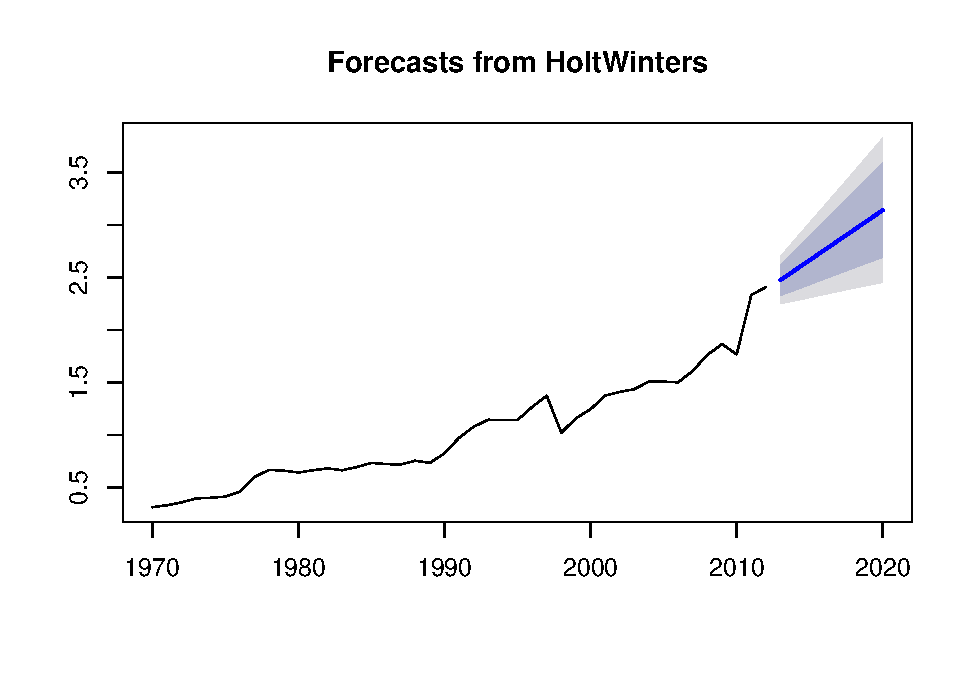
\includegraphics{dv_files/figure-latex/unnamed-chunk-67-1.pdf}

\hypertarget{using-themes}{%
\subsubsection{Using Themes}\label{using-themes}}

We can spice up our visualizations using another nifty feature of
\texttt{ggplot}: themes! I've copied and pasted the code from our
earlier exercise and added a theme using \texttt{theme\_linedraw()}. I
invite you to go ahead and swap out the theme and replace it with one of
the other themes. Examples:\\
- \texttt{theme\_calc()}\\
- \texttt{theme\_excel()} - \texttt{theme\_gdocs()}\\
- \texttt{theme\_classic()}

\begin{Shaded}
\begin{Highlighting}[]
\KeywordTok{ggplot}\NormalTok{(temp1, }\KeywordTok{aes}\NormalTok{(}\DataTypeTok{x=}\NormalTok{Var1, }\DataTypeTok{y=}\NormalTok{Freq))}\OperatorTok{+}
\StringTok{  }\KeywordTok{geom_col}\NormalTok{()}\OperatorTok{+}
\StringTok{  }\KeywordTok{theme_linedraw}\NormalTok{()}\OperatorTok{+}
\StringTok{  }\KeywordTok{labs}\NormalTok{(}\DataTypeTok{title=}\StringTok{"Most Represented Channels among Trending Videos"}\NormalTok{)}\OperatorTok{+}
\StringTok{  }\KeywordTok{theme}\NormalTok{(}\DataTypeTok{axis.text.x =} \KeywordTok{element_text}\NormalTok{(}\DataTypeTok{angle =} \DecValTok{90}\NormalTok{, }\DataTypeTok{hjust =} \DecValTok{1}\NormalTok{))}
\end{Highlighting}
\end{Shaded}

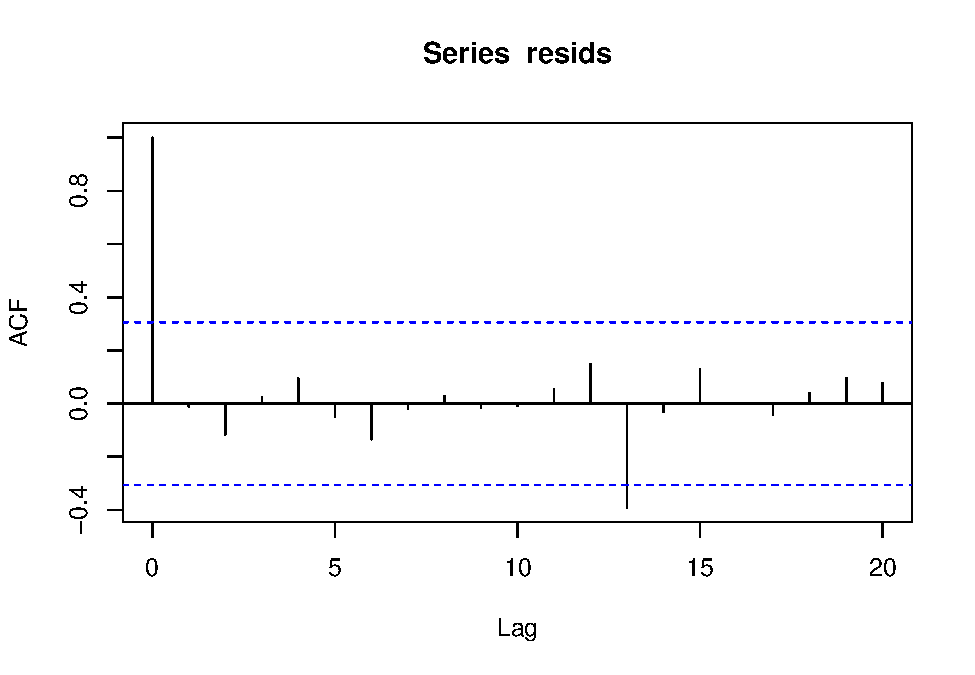
\includegraphics{dv_files/figure-latex/unnamed-chunk-68-1.pdf}

Now try one more example - try and replace \texttt{theme\_wsj} with one
of the other themes in the following plot. A simple switch of the
overall presentation ``theme'' using a short function like
\texttt{theme\_} makes it easy to experiment with different aesthetics
and is one of yet another benefit of using ggplot!

\begin{Shaded}
\begin{Highlighting}[]
\KeywordTok{ggplot}\NormalTok{(}\DataTypeTok{data =}\NormalTok{ vids.ags, }\KeywordTok{aes}\NormalTok{(}\DataTypeTok{x=}\NormalTok{category_id, }\DataTypeTok{y=}\NormalTok{dislikes, }\DataTypeTok{size=}\NormalTok{comment_count}\OperatorTok{/}\NormalTok{views))}\OperatorTok{+}
\StringTok{  }\KeywordTok{geom_jitter}\NormalTok{(}\KeywordTok{aes}\NormalTok{(}\DataTypeTok{col=}\NormalTok{publish_wday))}\OperatorTok{+}
\StringTok{  }\KeywordTok{theme_wsj}\NormalTok{(}\DataTypeTok{base_size =} \DecValTok{8}\NormalTok{)}\OperatorTok{+}
\StringTok{  }\KeywordTok{labs}\NormalTok{(}\DataTypeTok{title =} \StringTok{"Trending Videos Between 3 Categories"}\NormalTok{)}\OperatorTok{+}
\StringTok{  }\KeywordTok{theme}\NormalTok{(}\DataTypeTok{legend.position =} \StringTok{"none"}\NormalTok{)}
\end{Highlighting}
\end{Shaded}

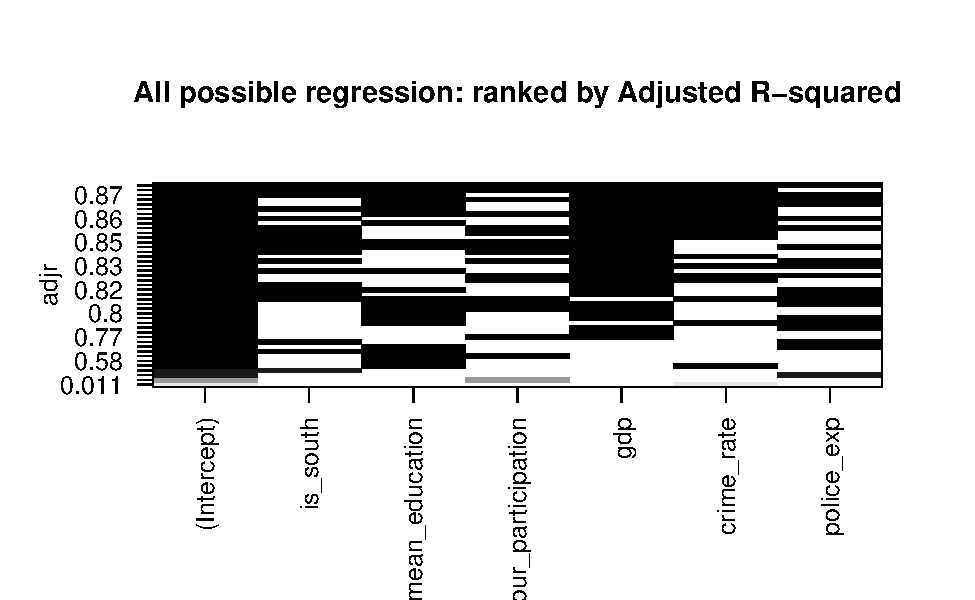
\includegraphics{dv_files/figure-latex/unnamed-chunk-69-1.pdf}

\hypertarget{introduction-to-leaflet-optional}{%
\subsection{Introduction to Leaflet
{[}Optional{]}}\label{introduction-to-leaflet-optional}}

Leaflet is among the most popular JS library for interative maps, used
by websites such as The New York Times, The Washington Post, GitHub and
Flickr\footnote{Official Documentation, Leaflet}. The R package
\texttt{leaflet} allows us to create leaflet maps directly in R code.
The steps are as follow:

\begin{enumerate}
\def\labelenumi{\arabic{enumi}.}
\tightlist
\item
  Create a map widget by calling leaflet().\\
\item
  Add layers (i.e., features) to the map by using layer functions
  (\texttt{addTiles}, \texttt{addMarkers}, \texttt{addPolygons}) to
  modify the map widget.
\end{enumerate}

Sounds similar enough to the ggplot system? Let's see a simple example.

I'm going to create two objects to be used for our Leaflet map later.
First, an icon! Here I'm using Algoritma's main icon and saving it to an
object called \texttt{ico}. Next, we'll create \texttt{loca}, a data
frame that has two variables (\texttt{lat} and \texttt{lng}) with some
randomly generated numbers. The code is straightforward:

\begin{Shaded}
\begin{Highlighting}[]
\KeywordTok{set.seed}\NormalTok{(}\DecValTok{418}\NormalTok{)}
\KeywordTok{library}\NormalTok{(leaflet)}

\NormalTok{ico <-}\StringTok{ }\KeywordTok{makeIcon}\NormalTok{(}
    \DataTypeTok{iconUrl =} \StringTok{"https://algorit.ma/wp-content/uploads/2017/07/logo_light_trans.png"}\NormalTok{,}
    \DataTypeTok{iconWidth=}\DecValTok{177}\OperatorTok{/}\DecValTok{2}\NormalTok{, }\DataTypeTok{iconHeight=}\DecValTok{41}\OperatorTok{/}\DecValTok{2}
\NormalTok{)}


\NormalTok{loca <-}\StringTok{ }\KeywordTok{data.frame}\NormalTok{(}\DataTypeTok{lat=}\KeywordTok{runif}\NormalTok{(}\DecValTok{5}\NormalTok{, }\DataTypeTok{min =} \FloatTok{-6.24}\NormalTok{, }\DataTypeTok{max=}\OperatorTok{-}\FloatTok{6.23}\NormalTok{),}
                   \DataTypeTok{lng=}\KeywordTok{runif}\NormalTok{(}\DecValTok{5}\NormalTok{, }\DataTypeTok{min=}\FloatTok{106.835}\NormalTok{, }\DataTypeTok{max=}\FloatTok{106.85}\NormalTok{))}
\end{Highlighting}
\end{Shaded}

And we'll now create our map:

\begin{Shaded}
\begin{Highlighting}[]
\CommentTok{# create a leaflet map widget}
\NormalTok{map1 <-}\StringTok{ }\KeywordTok{leaflet}\NormalTok{()}

\CommentTok{# add tiles from open street map}
\NormalTok{map1 <-}\StringTok{ }\KeywordTok{addTiles}\NormalTok{(map1)}

\CommentTok{# add markers}
\NormalTok{map1 <-}\StringTok{ }\KeywordTok{addMarkers}\NormalTok{(map1, }\DataTypeTok{data =}\NormalTok{ loca, }\DataTypeTok{icon=}\NormalTok{ico)}

\NormalTok{map1}
\end{Highlighting}
\end{Shaded}

\hypertarget{htmlwidget-e10917d6bbe247ef6956}{}
\begin{leaflet}

\end{leaflet}

Supposed we want the end user to be able to click on each of these icons
and have a simple pop-up description, we can add that to our map too!

Create the pop-up text:

\begin{Shaded}
\begin{Highlighting}[]
\NormalTok{pops <-}\StringTok{ }\KeywordTok{c}\NormalTok{(}
    \StringTok{"<h3>Algoritma Main HQ</h3><p>Visit us here!</p>"}\NormalTok{,}
    \StringTok{"<strong>Algoritma Business Campus</strong>"}\NormalTok{, }
    \StringTok{"<h3>In-Construction</h3><p>New Secondary Campus</p>"}\NormalTok{,}
    \StringTok{"<strong>Secondary Campus</strong>"}\NormalTok{,}
    \StringTok{"<strong>The Basecamp (business-school)</strong>"}
\NormalTok{)}
\end{Highlighting}
\end{Shaded}

Adding them to our map:

\begin{Shaded}
\begin{Highlighting}[]
\NormalTok{map1 <-}\StringTok{ }\KeywordTok{leaflet}\NormalTok{()}
\NormalTok{map1 <-}\StringTok{ }\KeywordTok{addTiles}\NormalTok{(map1)}
\NormalTok{map1 <-}\StringTok{ }\KeywordTok{addMarkers}\NormalTok{(map1, }\DataTypeTok{data =}\NormalTok{ loca, }\DataTypeTok{icon=}\NormalTok{ico, }\DataTypeTok{popup =}\NormalTok{ pops)}

\NormalTok{map1}
\end{Highlighting}
\end{Shaded}

\hypertarget{htmlwidget-89ba7edd121b3573cac8}{}
\begin{leaflet}

\end{leaflet}

\texttt{leaflet} does a lot more than the simple demonstration above,
but since it belongs to the optional part of this coursebook - I'll
leave it up to you, the readers, to further explore its possibilities!
While I would recommend you to use \texttt{ggplot} as the main focus of
your graded assignment, I want to leave the choice up to you. Work with
your academic mentors to produce a visualization as specified in the
learn-by-building module and good luck!

\hypertarget{summary}{%
\section{Summary}\label{summary}}

The coursebook covers many aspects of plotting, including using
visualization libraries such as \texttt{ggplot2}, \texttt{leaflet} and a
few other supporting libraries. I hope you've managed to get a good
grasp of the plotting philosophy behind \texttt{ggplot2}, and have built
a few visualizations with it yourself!

Happy coding!

Samuel

\hypertarget{annotations}{%
\subsection{Annotations}\label{annotations}}

Cleveland (1985), page 264: ``Data that can be shown by pie charts
always can be shown by a dot chart. This means that judgements of
position along a common scale can be made instead of the less accurate
angle judgements.'' This statement is based on the empirical
investigations of Cleveland and McGill as well as investigations by
perceptual psychologists."

\end{document}
